\chapter{Keyboard Design} \label{keyboard_design}

\section{Word-gesture Keyboard Implementation}
\subsection{Lacking Word-recognition} \label{lacking_word_recognition}
Recreating a word-gesture keyboard from scratch with the limited, non-commercial information available was considered to be outside of the scope of this thesis. Word-recognition has already been proven to work and benefits word-gesture keyboards, including mid-air, by providing high recognition rates of word-gesture shapes (e.g., low error rate and high text-entry rates) \cite{ref_shape_writing,ref_the_word_gesture_keyboard,ref_shapewriter_iphone,ref_shark_wgk,ref_shorthand_writing,ref_vulture}. Word-recognition is a requirement for traditional word-gesture keyboards because the intended word-gestures that are being generated are \textit{unknown}. However, the word-gestures that were generated in this thesis were \textit{known} in advance. Because the software has preexisting knowledge of the intended word-gesture shapes, it was concluded that word-recognition was not absolutely necessary to build a fully featured word-gesture keyboard. Therefore, a pseudo word-gesture keyboard implementation based on the presented gesture-shapes was used.

Using a pseudo word-gesture keyboard implementation presented its own challenges and limitations. One possible limitation was that character production, including detected errors, occurred mid-gesture. This meant that participants were more likely to stop mid-gesture and interrupt the gesturing-process to correct errors rather than following through with the full word-gesture shape as in traditional word-gesture keyboards. This was expected to slow text-entry rates. Another possible issue was that since the pseudo word-gesture keyboard did not implement shape-recognition, the gesture-path had to be analyzed as it was being drawn. Therefore, key ``presses'' had to be interpreted through path changes or by the user passing through the expected key. Section~\ref{design} explains how this works in greater detail. Lacking shape-recognition could lead to higher error rates. Additionally, because gesture-shapes were not recognized against a compendium of common words, these limitations allowed user-generation of non-words (e.g., words not in any dictionary). Although these limitations existed, the results of this thesis can be extrapolated to traditional word-gesture keyboards. This claim is justified by the Leap Pinch-air Keyboard ($M = 11.3$ WPM) performing consistently with the pinching-method from Vulture ($M = 11.8$ WPM) for text-entry rates in a single session with no training \cite{ref_vulture}. Additionally, the Leap Pinch-air Keyboard reached 58\% of the text-entry rate of direct touch input, which was proportional to Vulture at 59\% of the text-entry rate of direct touch input \cite{ref_vulture}. Many of these changes and limitations occurred on the back-end (software) while still presenting a similar experience for the user to traditional word-gesture keyboards.

\subsection{Design} \label{design}
The pseudo word-gesture implementation was created by analyzing the user's generated gesture compared to the expected gesture as it was being drawn to determine which keys were being pressed. The assumptions for detecting a key press were based off the known word being gestured and noticeable deviations made in the gesture's direction. To reduce the chance of erroneous keys being pressed, the sizes of the characters expected to be pressed were exaggerated and the deviation threshold in gestures were lowered between key paths.

The displayed keys were 64x64 pixels in size with a gap of 10 pixels between each key. The actual size of the keys was dependent on the display device being used. The next expected letter to be pressed in a word was changed into a circular key with a radius of 76.8 pixels, 20\% larger than the key widths, in order to make hitting keys even easier. Figure~\ref{key_bloating} shows how keys were changed behind the scenes. However, the software presented no visual feedback to the participant of the increased key sizes.

\begin{figure}[!t]
	\centering
	\includegraphics[width=5in]{Figures/fig_bloat_key}
	\caption[Larger Key Example]{The next expected key to be pressed was increased in size to make pressing it easier. The above visual shows how it was interpreted by the software, but there was no visual feedback presented to users.}
	\label{key_bloating}
\end{figure}

An interpolated trail with points at a minimum of 16 pixels apart was used in determining deviations in word-gesturing. The angle of detecting a deviation was 165 degrees for all areas that were not on the expected path to the next key and was 90 degrees while on the expected path. Deviations in gesture path had to be at least 48 pixels away from each other to be counted as a ``press''. The expected path between two keys comprised an area from the previous expected key to the next expected key with a width 62.5\% larger than key size, or 104 pixels. Figure~\ref{protected_path} shows how the expected path protects against natural deviations when moving from one key to the next.

\begin{figure}[!t]
	\centering
	\begin{minipage}[t]{3in}
		\includegraphics[width=2.5in]{Figures/fig_path_no_protection}
		\subcaption{No Path Protection\ \ \ \ \ \ \ \ \ }
	\end{minipage}
	\begin{minipage}[t]{2.5in}
		\includegraphics[width=2.5in]{Figures/fig_path_no_error}
		\subcaption{Path Protection}
	\end{minipage}
	\begin{minipage}[t]{2.5in}
		\includegraphics[width=2.5in]{Figures/fig_path_with_error}
		\subcaption{Error with Path Protection}
	\end{minipage}
	\caption[Protected Path Example]{A path between the currently pressed letter and the next letter significantly reduces the chance of detecting erroneous input. (a) shows an error detected with an angle less than 165 degrees; (b) shows how as long as the user stayed on the path, errors were significantly reduced; and (c) shows that errors could still be detected on a protected path if a deviation with an angle less than 90 degrees was detected.}
	\label{protected_path}
\end{figure}

The specific values for detecting key presses were found using trial and error. These were used to create an experience as close to a traditional word-gesture keyboard as possible. Whereas the word-recognition implementation showed the transcribed word after the completed gesture, the pseudo-implementation showed participants real-time updates of detected character presses along the keyboard path. This was determined to be an acceptable limitation as explained in Section~\ref{lacking_word_recognition}.

\subsection{Display}
\subsubsection{Keyboard layout}
The keyboard layout, seen in Figure~\ref{keyboard_layout}, was a typical QWERTY keyboard with key sizes of 64x64 pixels and gaps of 10 pixels. All special keys and number keys were removed to simplify the keyboard and a backspace key added to the keyboard's right side to allow for erroneous character deletion.

\begin{figure}[t]
	\centering
	\includegraphics[width=6in]{Figures/fig_final_keyboard}
	\caption[Display: Keyboard Layout]{The keyboard layout used during the full study.}
	\label{keyboard_layout}
\end{figure}

\subsubsection{Text area}
Figure~\ref{text_area} shows how two text areas were used to display text to participants. The top text-area displayed a presented word, shown in Figure~\ref{text_a}, and the bottom text-area displayed the presented word's transcription, shown in Figure~\ref{text_b}. Both the presented word and transcription's characters were colored green when correctly matched. If errors were made during transcription, only characters in the transcribed text would display in red. The participant could then use the backspace to correct errors. When the transcription matched the presented word, both text-areas were highlighted in green, as seen in Figure~\ref{text_c}.

\begin{figure}[!b]
	\centering
	\begin{minipage}[t]{1.9in}
		\includegraphics[width=2in]{Figures/fig_idle_keyboard}
		\subcaption{Displayed Word}
		\label{text_a}
	\end{minipage}
	\begin{minipage}[t]{1.9in}
		\includegraphics[width=2in]{Figures/fig_error_keyboard}
		\subcaption{Transcribed Error}
		\label{text_b}
	\end{minipage}
	\begin{minipage}[t]{1.9in}
		\includegraphics[width=2in]{Figures/fig_correct_keyboard}
		\subcaption{Completed Word}
		\label{text_c}
	\end{minipage}
	\caption[Display: Text Area]{Examples of how the text areas change when showing transcribed text. (a) shows the word to be transcribed as it first appears; (b) shows how correct letters were colored green in both text areas and transcription errors were colored red; and (c) shows the user-generated text and presented word highlighted to indicate correct transcription.}
	\label{text_area}
\end{figure}

\subsubsection{Real-time updates}
As a participant was drawing the gesture-shape of a word, their progress was tracked in real-time, as shown in Figure~\ref{display_area}. For the keyboards that tracked a finger or stylus, the software displayed a cylinder to indicate the input's position and direction in 3-dimensional space relative to the virtual keyboard as shown in Figure~\ref{update_a}. In addition, it displayed which letter the user's input hovered over by projecting a blue dot to the corresponding virtual keyboard location. As seen in Figure~\ref{update_b}, the software showed the participant the gesture-path that they were traveling in addition to the letters that had been pressed. The gesture-trail decayed over time in order to not clutter the display. 

\begin{figure}[!t]
	\centering
	\begin{minipage}[t]{2.9in}
		\includegraphics[width=3in]{Figures/fig_update1_keyboard}
		\subcaption{Prior to pressing `d'}
		\label{update_a}
	\end{minipage}
	\begin{minipage}[t]{2.9in}
		\includegraphics[width=3in]{Figures/fig_update2_keyboard}
		\subcaption{During the word-gesture}
		\label{update_b}
	\end{minipage}
	\caption[Display: Real-time Updates]{Examples of the real-time display for word-gesturing. (a) shows the user just about to press the first character; and (b) shows the word gesturing process for the word ``decent.''}
	\label{display_area}
\end{figure}

\subsection{Calibration}
Each mid-air keyboard, and the Leap Surface Keyboard, could be calibrated in a manner similar to Personal Space \cite{ref_alvin_thesis}, seen in Figure~\ref{calibration_in_progress}. Many of the calibration spaces, however, required direct interaction instead of projecting the inputs onto the interaction plane. Default calibrations were adequate for most participants, but recalibration was optional. However, calibration had less of a lasting effect because many participants repositioned the Leap Motion controller itself. Participants were encouraged to adjust the controller's position to promote usability. This was sometimes a greater factor than motor space calibration for translating precise movement to the virtual keyboard. Because this thesis was not an accessibility study, participants were allowed to calibrate the keyboard with their arms rested or raised. Therefore, this thesis did not address the ``Gorilla Arm Syndrome'' mentioned in Section~\ref{gorilla_arm_syndrome}.

\begin{figure}[!t]
	\centering
	\begin{minipage}[t]{4in}
		\begin{minipage}[t]{1.9in}
			\includegraphics[width=2in]{Figures/fig_calib_1}
		\end{minipage}
		\begin{minipage}[t]{1.9in}
			\includegraphics[width=2in]{Figures/fig_calib_2}
		\end{minipage}
	\end{minipage}
	
	\begin{minipage}[t]{4in}
		\begin{minipage}[t]{1.9in}
			\includegraphics[width=2in]{Figures/fig_calib_3}
		\end{minipage}
		\begin{minipage}[t]{1.9in}
			\includegraphics[width=2in]{Figures/fig_calib_4}
		\end{minipage}
	\end{minipage}
	\caption[Calibration]{Participants were able to follow on-screen instructions to calibrate the interaction space using their finger.}
	\label{calibration_in_progress}
\end{figure}

\subsubsection{Motor space and display space}
The researcher attempted to place the Leap Motion controller to adjust the calibrated interaction plane, or the motor space, to be as parallel to the screen, or display space, as possible. However, participants were allowed to adjust the Leap Motion controller to a position that felt most comfortable to them. Moving the controller typically resulted in the motor space being oriented perpendicular to a participant's arm rather than parallel to the display space. Also to note, when working with keyboards that fully utilized the 3rd-dimension, an interaction plane angled away from a participant was sometimes more effective than a straight plane perpendicular to the floor. Figure~\ref{plane_angle} shows the difference between a straight plane and angled plane.

\begin{figure}[!t]
	\centering
	\begin{minipage}[t]{4in}
		\begin{minipage}[t]{1.9in}
			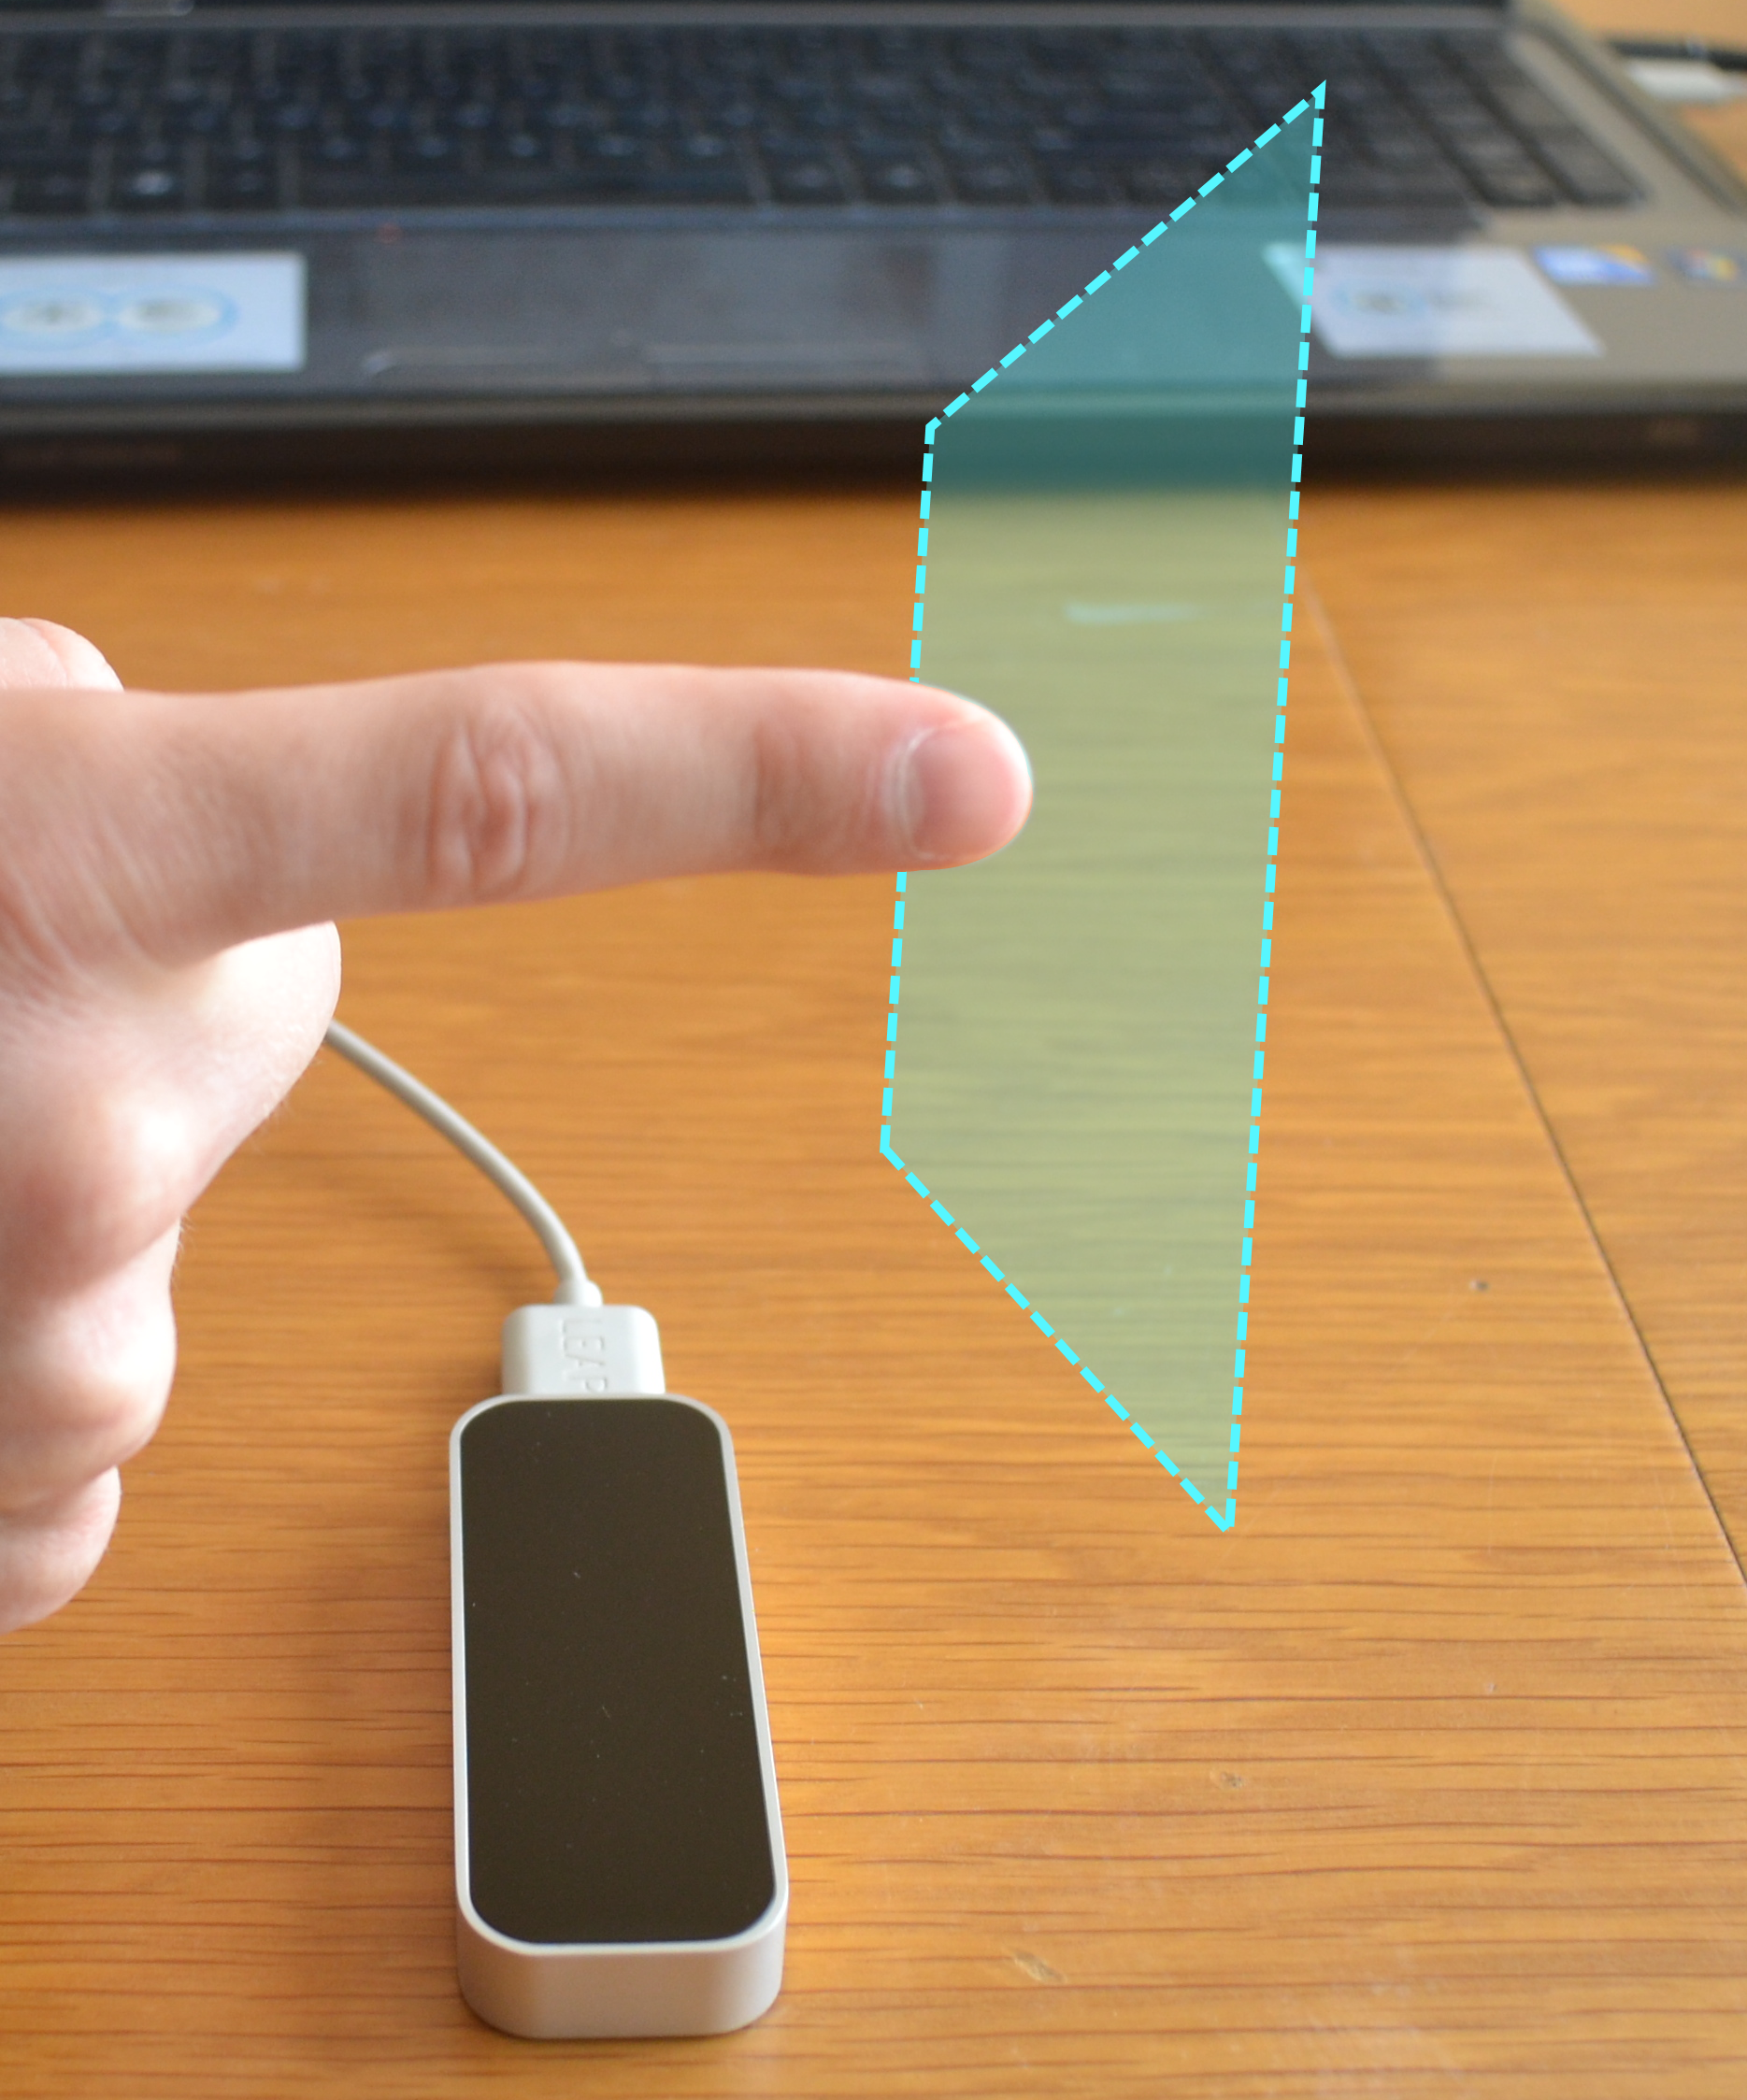
\includegraphics[width=2in]{Figures/fig_plane_straight}
			\subcaption{Straight Plane}
		\end{minipage}
		\begin{minipage}[t]{1.9in}
			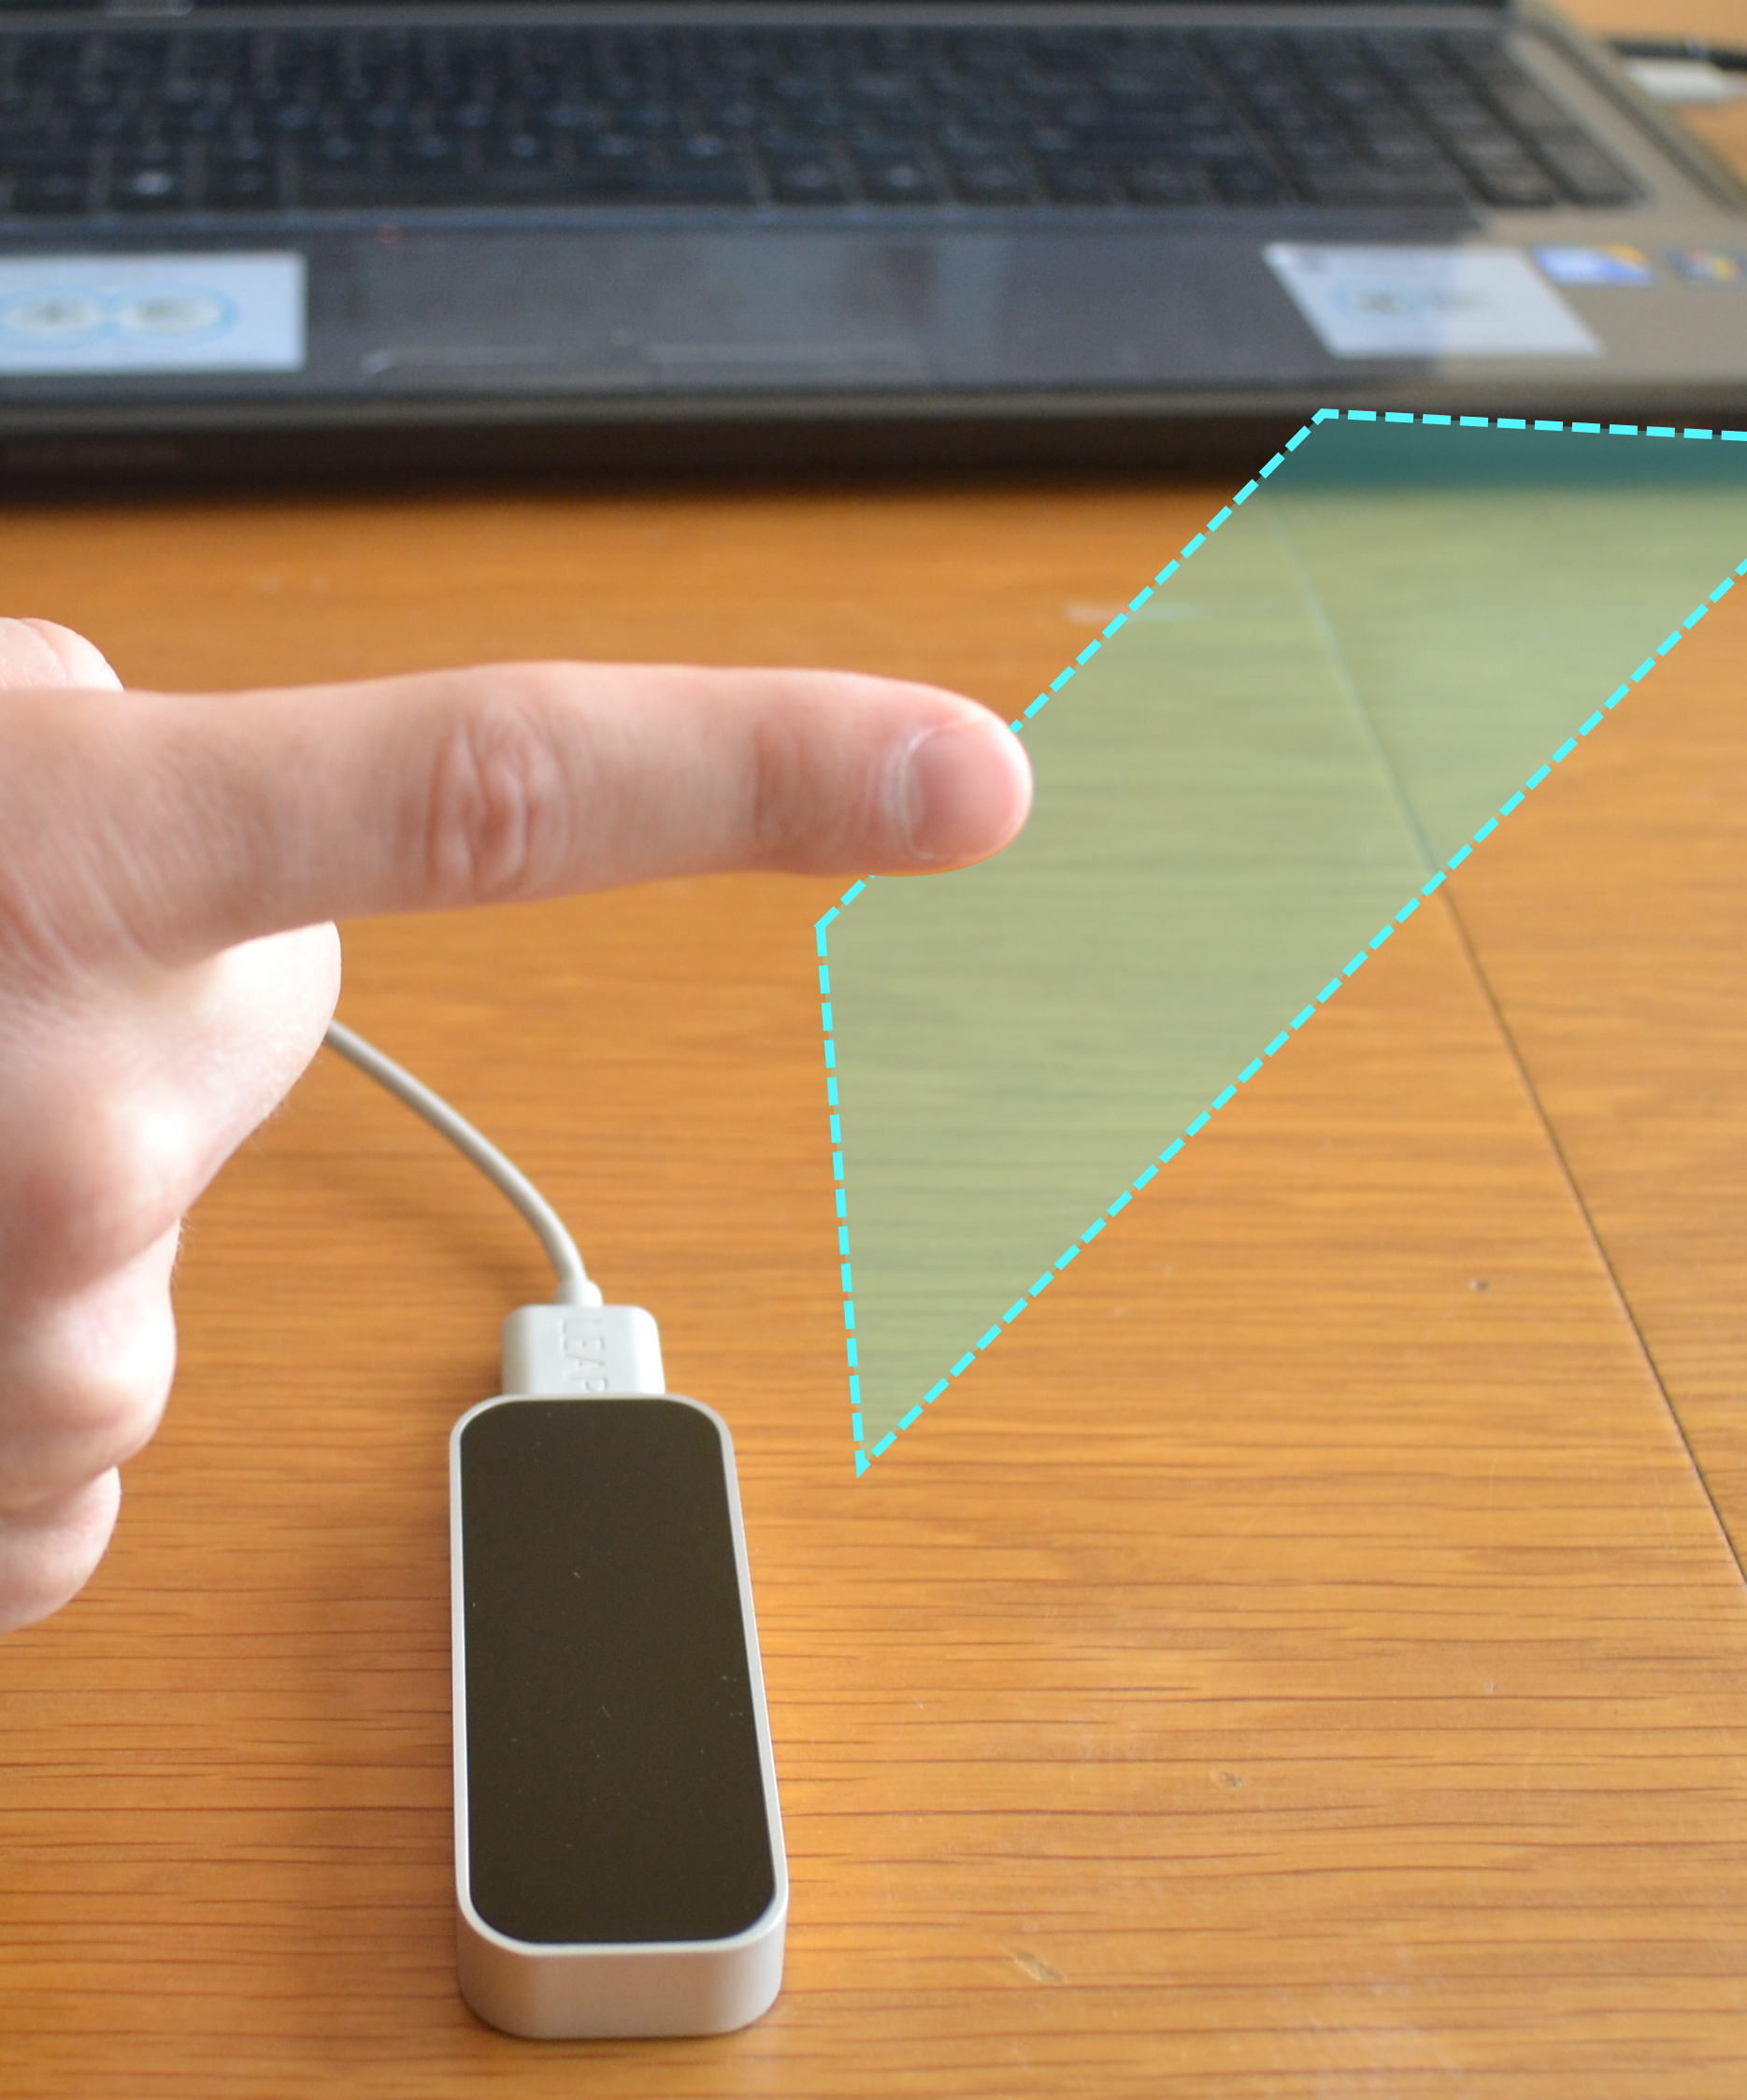
\includegraphics[width=2in]{Figures/fig_plane_angled}
			\subcaption{Angled Plane}
		\end{minipage}
	\end{minipage}
	\caption[Angled Plane]{Examples of a straight plane versus an angled plane.}
	\label{plane_angle}
\end{figure}

The size of the motor space was dependent on either the device the keyboard was presented on or the calibration of the keyboard's interaction plane. For all of the keyboards, the motor space was mapped to a display space of 952x212 pixels and keys that were 64x64 pixels with gaps of 10 pixels. The real-world size of the keyboard display was dependent on the screen being used. Figure~\ref{motor_space_size} shows the average sizes of the motor spaces.

\begin{figure}[!t]
	\centering
	\begin{minipage}[t]{2.5in}
		\includegraphics[width=2.5in]{Figures/fig_calibration_touch}
		\subcaption{Touch Screen}
		\label{fig_calibration_touch}
	\end{minipage}
	\begin{minipage}[t]{2.5in}
		\includegraphics[width=2.5in]{Figures/fig_calibration_surface}
		\subcaption{Leap Surface}
		\label{fig_calibration_surface}
	\end{minipage}
	\begin{minipage}[t]{2.5in}
		\includegraphics[width=2.5in]{Figures/fig_calibration_static}
		\subcaption{Static/Predictive/Bimodal}
		\label{fig_calibration_static}
	\end{minipage}
	\begin{minipage}[t]{2.5in}
		\includegraphics[width=2.5in]{Figures/fig_calibration_pinch}
		\subcaption{Leap Pinch-air}
		\label{fig_calibration_pinch}
	\end{minipage}
	\caption[Motor Space Comparison]{The average size of the motor spaces for each keyboard with a gradient color scale showing the plane orientation. The closest areas are represented by \textit{yellow} and the farthest by \textit{blue}. (a) shows the standard Touch Sceen motor space; (b) shows the average calibration for the Leap Surface motor space; (c) shows the average calibration for the Leap Static-air, Predictive-air, and Bimodal-air motor spaces (a single calibration was typically used for all three); and (d) shows the average calibration for the Leap Pinch-air motor space.}
	\label{motor_space_size}
\end{figure}

\subsection{Dictionary Creation} \label{dictionary_creation}
For the purposes of this thesis, the term ``dictionary'' denotes the pool of words presented to the participant. To make each keyboard experience as similar as possible, a custom dictionary was created for each keyboard interaction style. While different words were used for each dictionary, the words were selected by using a custom gesture-shape dissimilarity algorithm. This algorithm minimized dissimilarity between word gesture-shapes as shown in Appendix~\ref{dictionary_sets}. The algorithm's results were further reduced to common words between 3 and 6 characters in length. These unique word sets became each keyboard's dictionary.

\subsubsection{Deviating from the standard phrases}
To evaluate text-entry, typically predefined phrases were generated and used \cite{ref_phrase_sets}. However, due to the limited number of trials and the abundance of different conditions, single words were chosen as opposed to randomly selecting from a compendium of predefined phrase sets. The goal was to create new word dictionaries, avoiding whole phrases to prevent confusing language, using a custom algorithm to minimize the dissimilarity of different gesture-shapes. No previous research existed on words with similar gesture-shapes, or their benefit, but this thesis's purposeful deviation created similar keyboard experiences to standardize results across many conditions and few trials.

\subsubsection {Gesture-shape dissimilarity} \label{gesture_shape_dissimilarity}
Originally, this thesis considered the Fr\'echet Distance to find similar word gesture-shapes using sets of words with minimal distance between each letter within a gesture-shape. While Fr\'echet Distance gave acceptable results, there were noticeable differences in \textit{some} of the gesture-shape sets. Figure~\ref{fig_words_frechet} demonstrates these differences, which appears to show more than one primary gesture-shape returning for the set.

\begin{figure}[!b]
	\centering
	\includegraphics[width=5in]{Figures/fig_words_frechet}
	\caption[Fr\'echet Word Set]{An example of a gesture-shape set generated by the Fr\'echet Distance algorithm: `crass', `creed', `crews', `feeds', `feted', `fetes'. The Fr\'echet Distance, at times, generated more than one gesture-shape pattern per word set.}
	\label{fig_words_frechet}
\end{figure}

In order to achieve gesture-shapes that were more similar than shapes found by the Fr\'echet Distance, the custom dissimilarity algorithm was created. The words were pulled from the Oxford English Dictionary. The dissimilarity between two words' gesture-shapes was defined by the formula
\begin{equation}
dissimilarity(P,\ Q) = \frac{\sum\limits_{i = 2}^{N} \frac{1}{2} \left(\left(\frac{\mid dist(P_{i},\ P_{i-1}) - dist(Q_{i},\ Q_{i-1})\mid}{max\ distance}\right) + \left(\frac{angle(P_{i} - P_{i-1},\ Q_{i} - Q_{i-1})}{\pi}\right)\right)}{N - 1}
\end{equation}
where $P$ and $Q$ were two words of $N$ characters in length, $i$ was a particular character of $P$ or $Q$, $P_i$ and $Q_i$ were the vector locations on the virtual keyboard, $max\ distance$ was the maximum distance between any two letters on the virtual keyboard, $dist(...)$ was the distance between two vector locations, and $angle(...)$ was the angle between two vectors. The dissimilarity formula generated values between the range [0, 1] and treated every pair of paths between two letters of two words with equal weight. The objective was then to find the sets of words with the lowest dissimilarity.

\section{Word-gesture Keyboards}
All of the word-gesture keyboards created used the same word-gesturing implementation but differentiated by their interaction method and how touch was handled as a delimiter between words.

\subsection{Touch Screen Keyboard}
\subsubsection{Interaction method}
The Touch Screen Keyboard was implemented to mirror the de facto method for word-gesture keyboards, which are generally touch-based. The user interacts directly with a touch screen surface.

\subsubsection{Word separation}
Figure~\ref{touch_screen_press_comparison} shows that word separation for the Touch Screen Keyboard worked in the same way as typical word-gesture keyboards for phones and tablets. Touch was simulated simply by pressing a finger against the surface, drawing the word-gesture, and then removing the finger from the surface.

\begin{figure}[h]
	\centering
	\begin{minipage}[t]{5.8in}
		\begin{minipage}[t]{2.85in}
			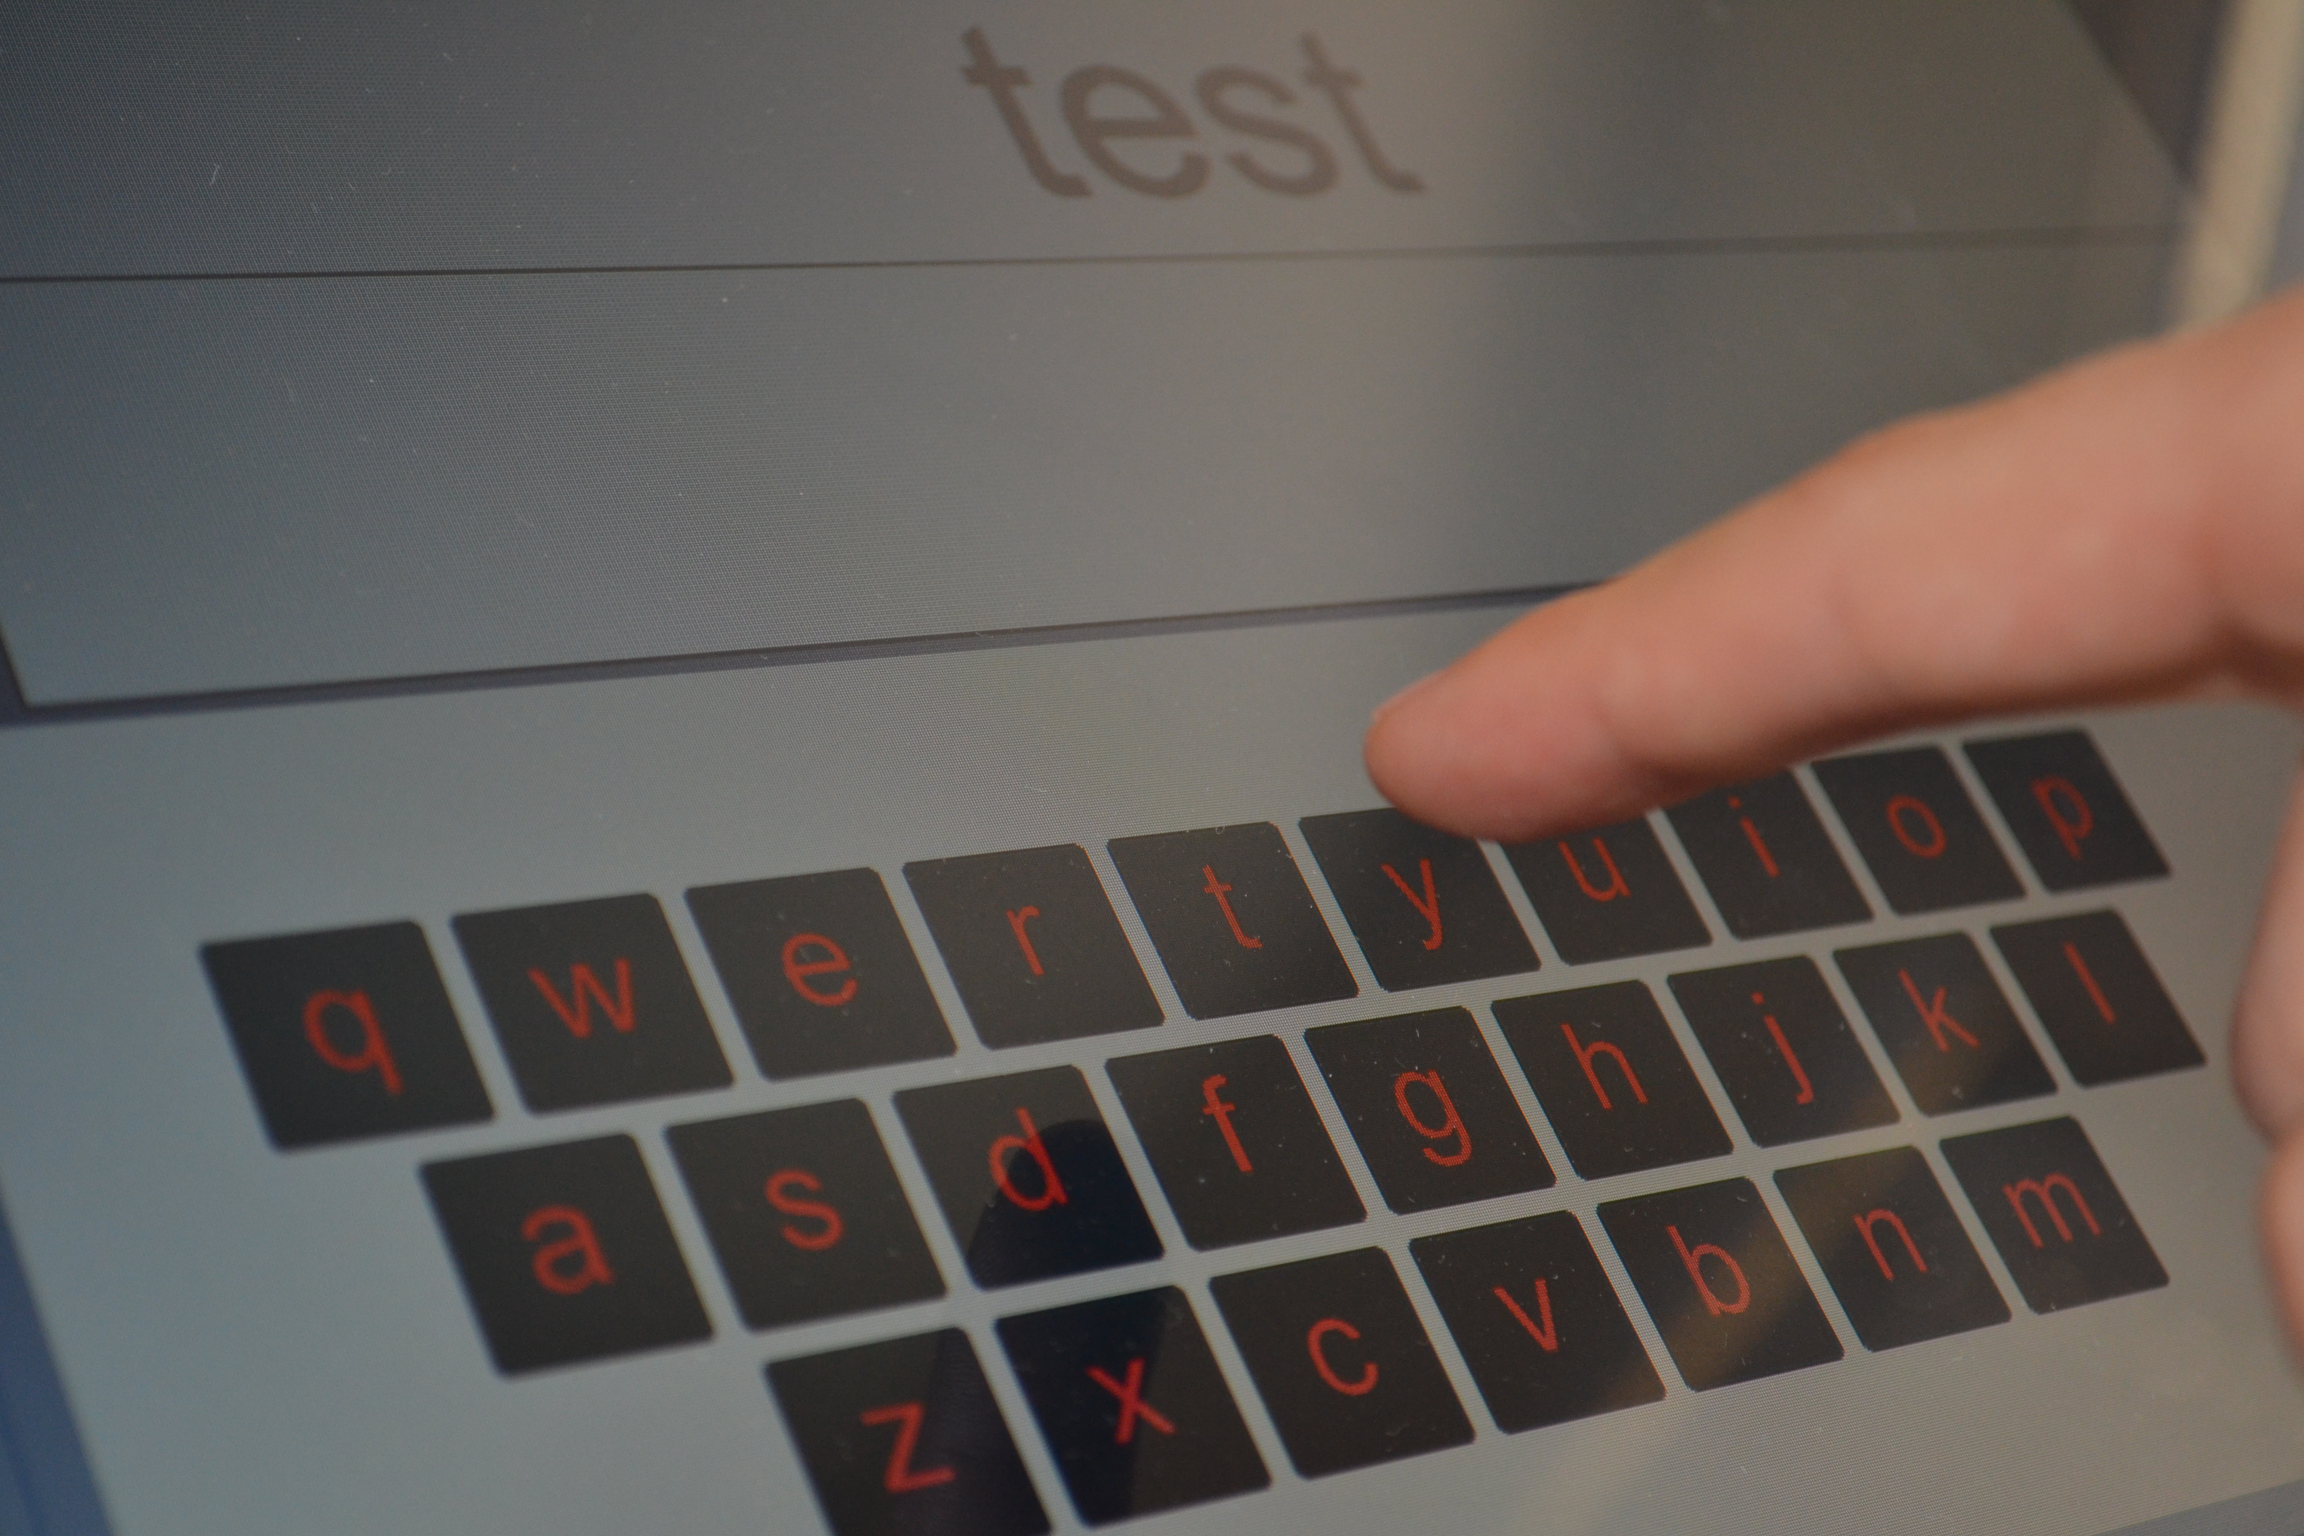
\includegraphics[width=2.9in]{Figures/fig_touch_screen_hover}
		\end{minipage}
		\begin{minipage}[t]{2.9in}
			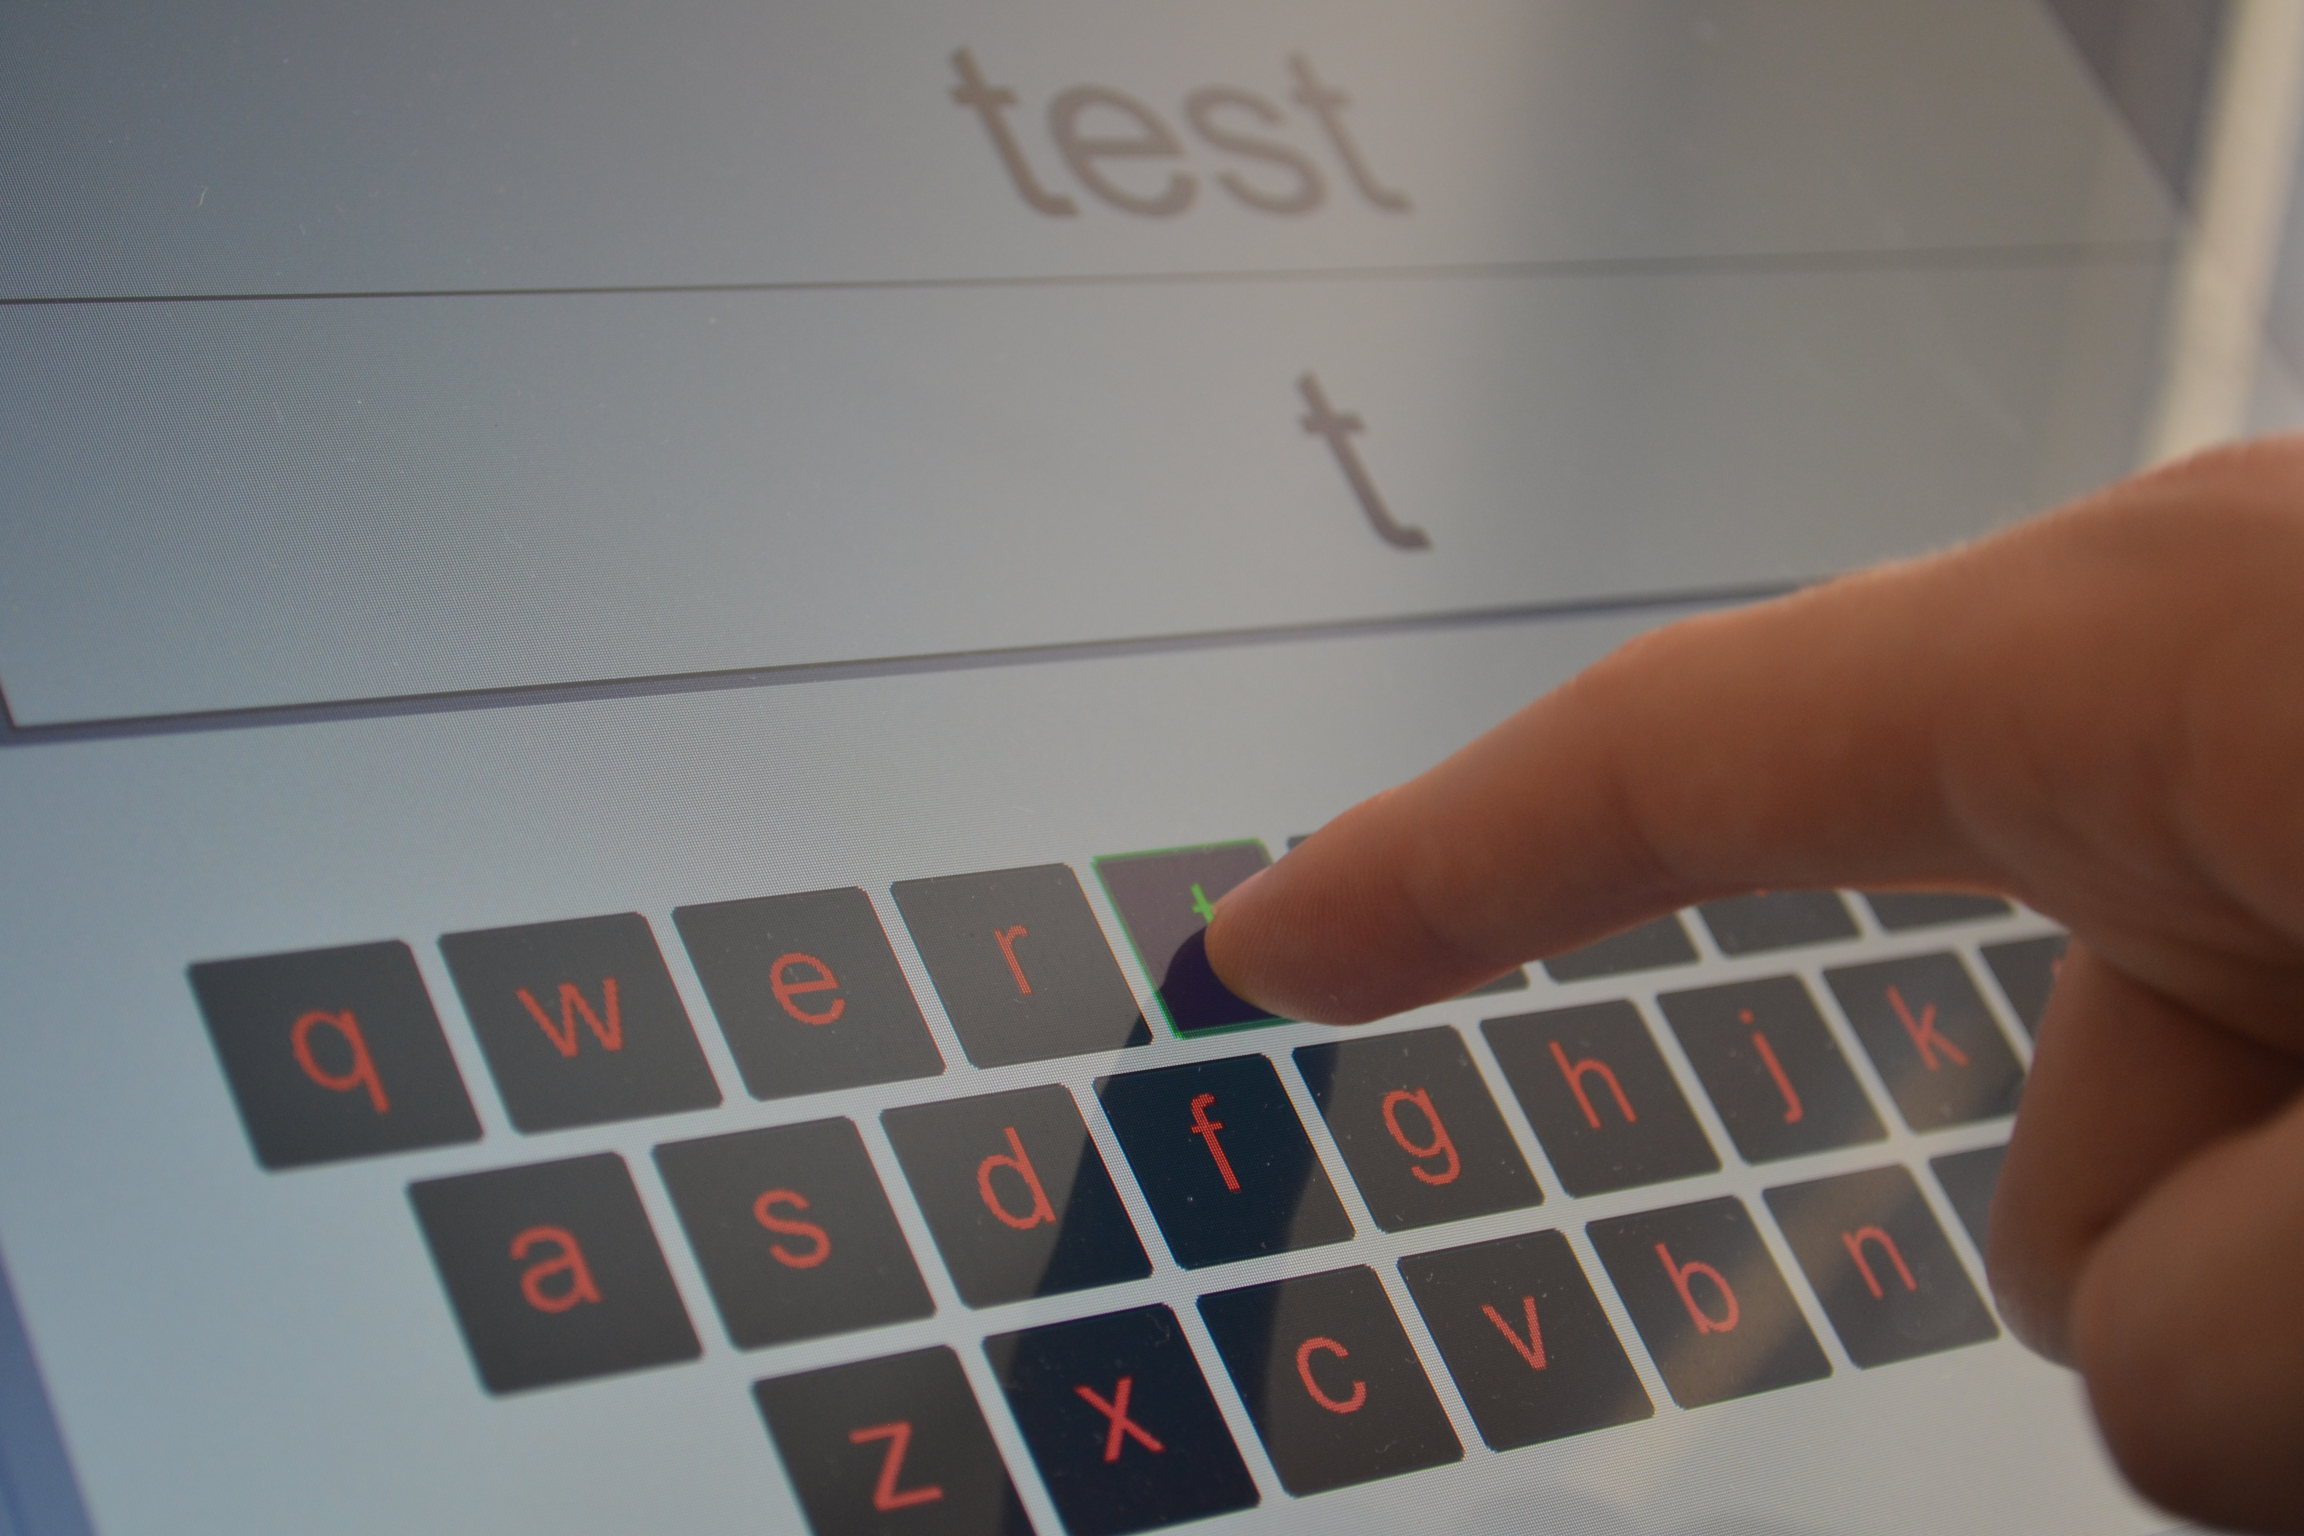
\includegraphics[width=2.9in]{Figures/fig_touch_screen_press}
		\end{minipage}
	\end{minipage}
	\caption[Touch Screen Word Separation]{A touch was simulated when the tabletop screen was touched with the user's pointer finger.}
	\label{touch_screen_press_comparison}
\end{figure}

\subsubsection{Size of the motor space}
The motor space for the Touch Screen Keyboard was larger than the other keyboard motor spaces because the display device was intrinsically larger and the Touch Screen's motor space and display space are coupled together. The display device used was a C4667PW boasting a $46^{\prime\prime}$ display space and a maximum resolution of 1920x1080 pixels. Figure~\ref{fig_3m_display} shows the C4667PW, a 3M\textsuperscript{TM} Multi-touch Display. When scaled for the maximum resolution, the Touch Screen display space and motor space were both 50.49x11.24 $cm$, with keys that were 3.39x3.39 $cm$ and gaps between keys of 0.53 $cm$. If higher resolutions were available, a higher resolution would have been chosen to decrease the overall size of the display space and motor space to match the other keyboards more closely. Though larger than desired, the 3M\textsuperscript{TM} Multi-touch Display was still preferred over using very small touch-based, word-gesture keyboards such as those on phones or tablets. A similar sized motor space helped standardize results between touch and mid-air.

\begin{figure}[!b]
	\centering
	\includegraphics[width=5in]{Figures/fig_3m_display}
	\caption[3M\textsuperscript{TM} Multi-touch Display]{The $46^{\prime\prime}$ C4667PW, a 3M\textsuperscript{TM} multi-touch tabletop display.}
	\label{fig_3m_display}
\end{figure}

\subsection{Leap Surface Keyboard} \label{leap_surface}
\subsubsection{Interaction method}
The Leap Surface Keyboard used the Leap Motion controller to track a wooden stylus for interaction. It was designed so that it would simulate a touch screen using a mid-air plane projected onto a surface. This was done by inserting the Leap Motion controller into a custom holder, shown in Figure~\ref{fig_leap_holder}, and projecting the mid-air keyboard over a keyboard printed on paper. As an added note, the Leap Surface Keyboard works in the exact same way as the Static-air Keyboard in Section~\ref{static_air} by being calibrated to a surface rather than mid-air. A stylus was chosen to be used as an interaction tool to allow for accurate surface emulation because the Leap Motion controller was in a position that made it difficult to successfully track a participants hand or finger. Unfortunately, the Leap Controller hardware, at the time of this thesis, was only designed to recognize hands from one direction, necessitating the controller be positioned at the bottom of the holder rather than the top.

\begin{figure}[h]
	\centering
	\includegraphics[width=5in]{Figures/fig_leap_holder}
	\caption[Leap Surface Holder]{The custom built holder, projecting an interaction plane onto a printed keyboard surface.}
	\label{fig_leap_holder}
\end{figure}

\subsubsection{Word separation}
Word separation for the Leap Surface Keyboard worked in a similar way to how touch was simulated using a stylus for a phone or tablet. Figure~\ref{leap_surface_press_comparison} shows how touch was simulated by pressing the tip of the stylus against the surface of the printed keyboard. The word-gestures were drawn and then the stylus removed from the surface to complete the action.

\begin{figure}[!t]
	\centering
	\begin{minipage}[t]{5.8in}
		\begin{minipage}[t]{2.85in}
			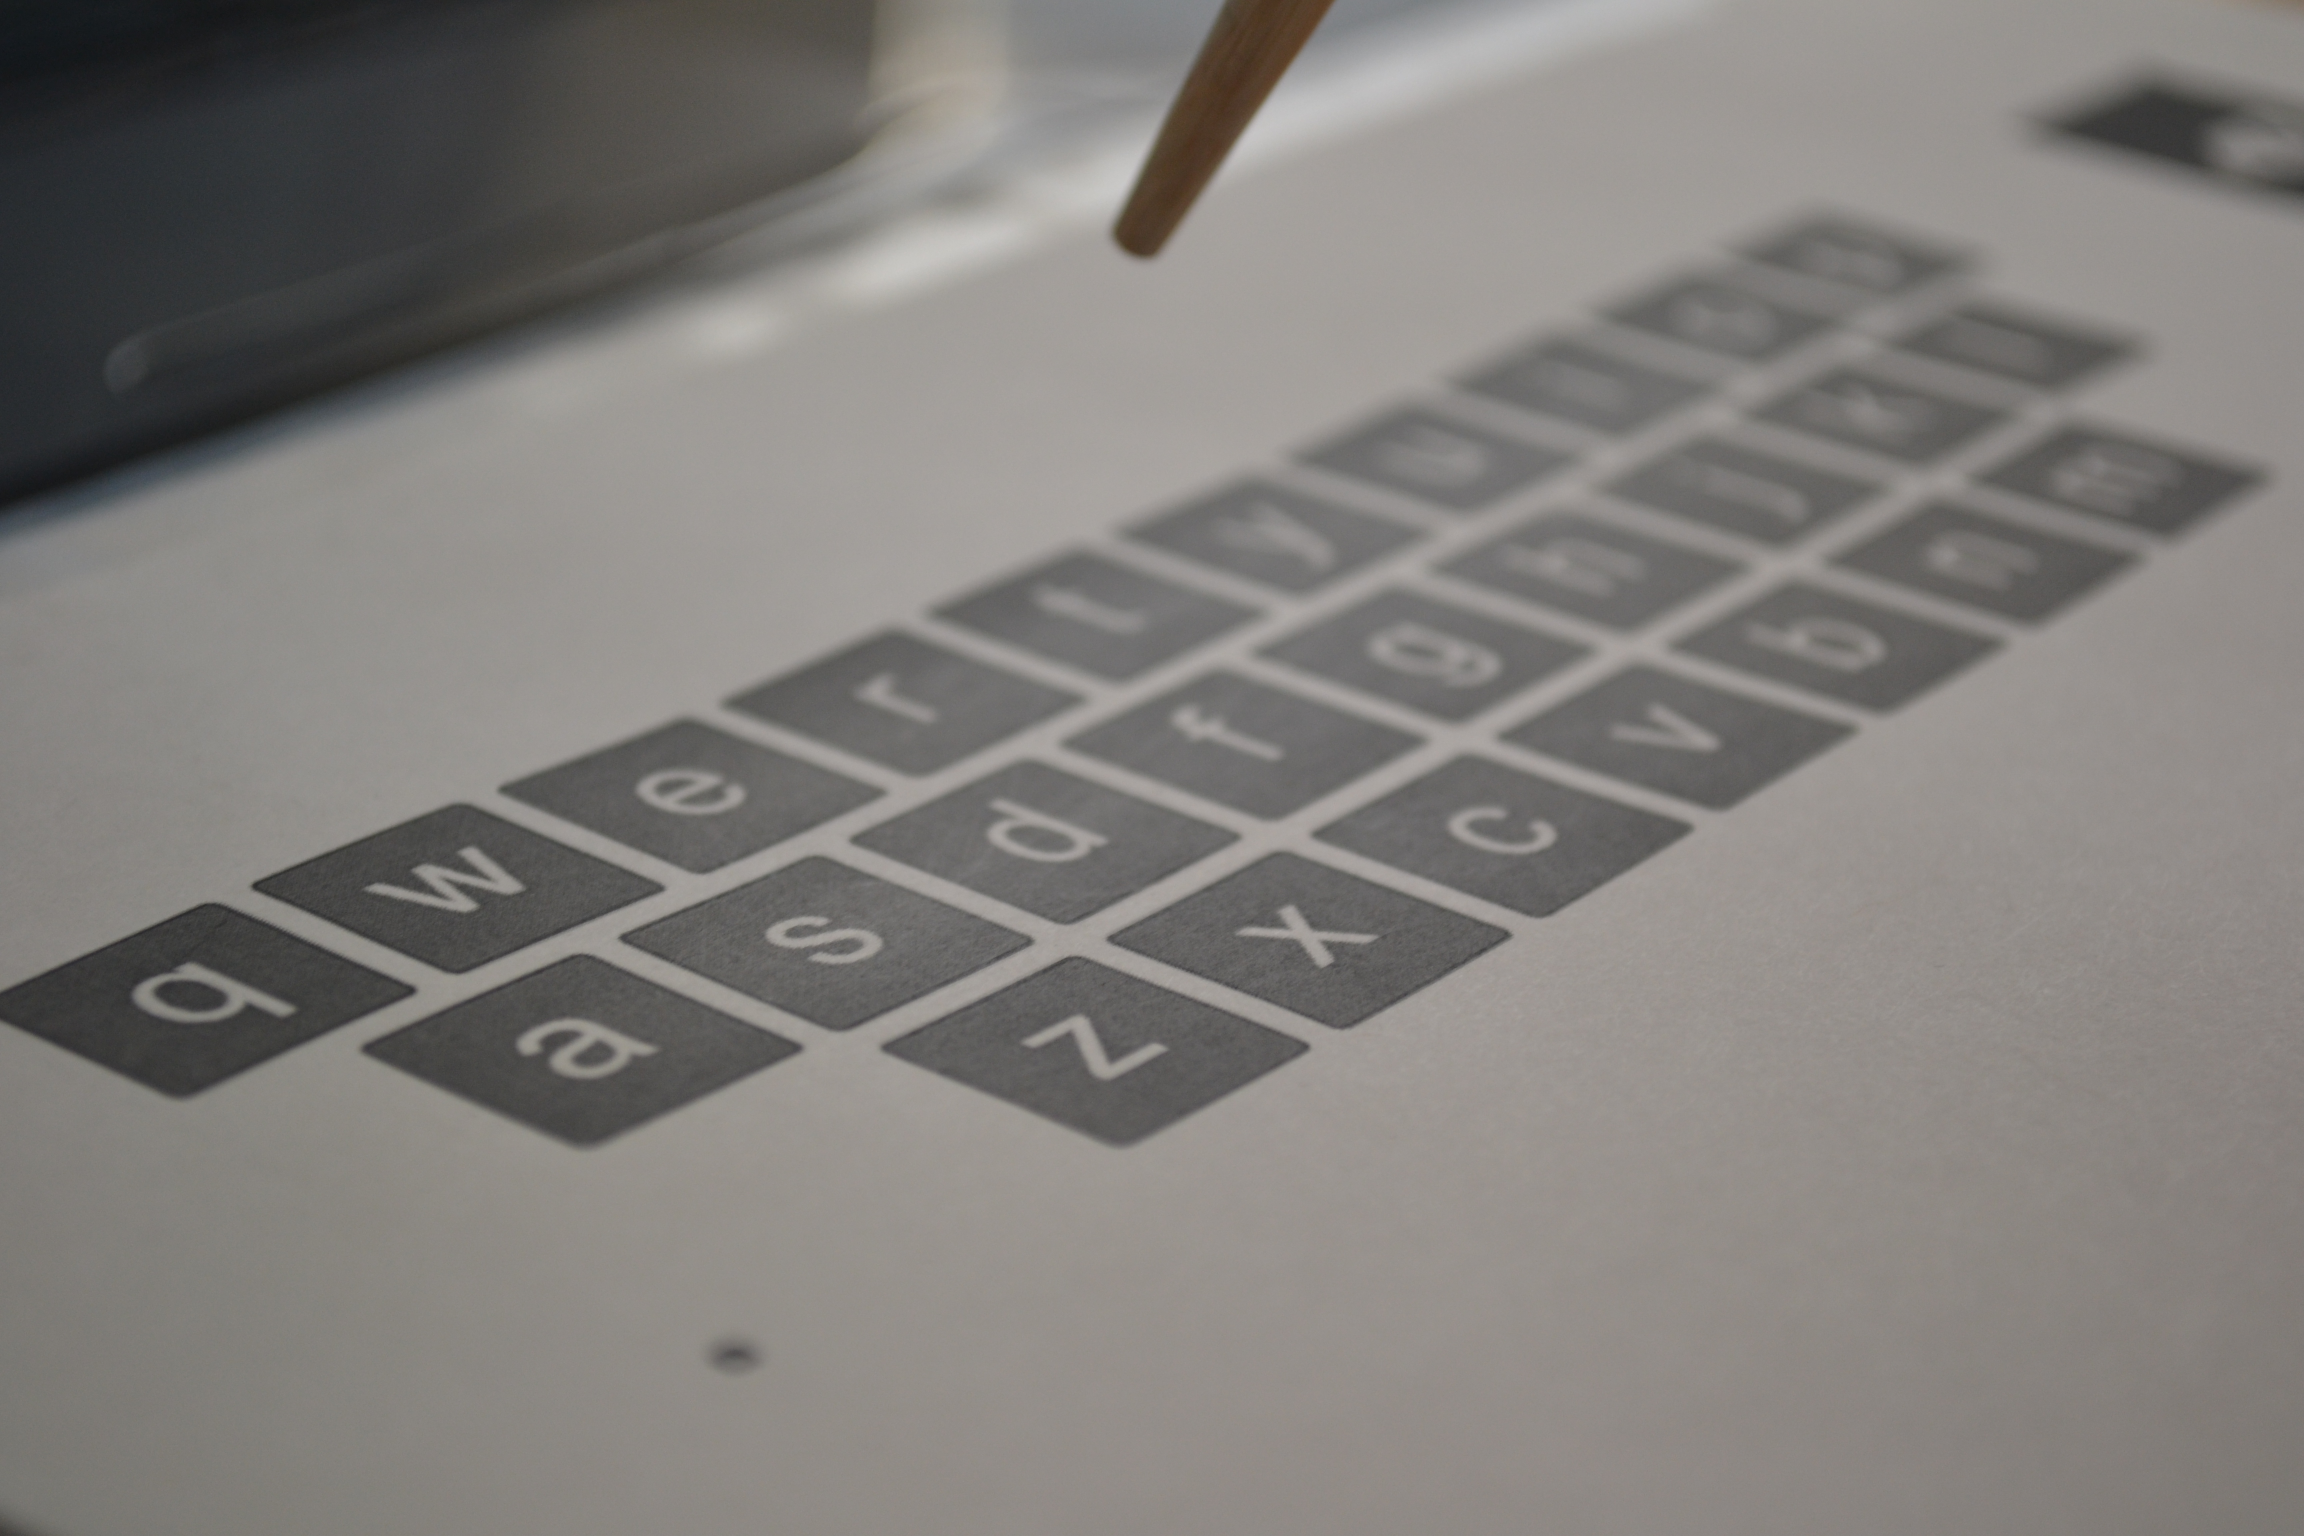
\includegraphics[width=2.9in]{Figures/fig_surface_hover}
		\end{minipage}
		\begin{minipage}[t]{2.9in}
			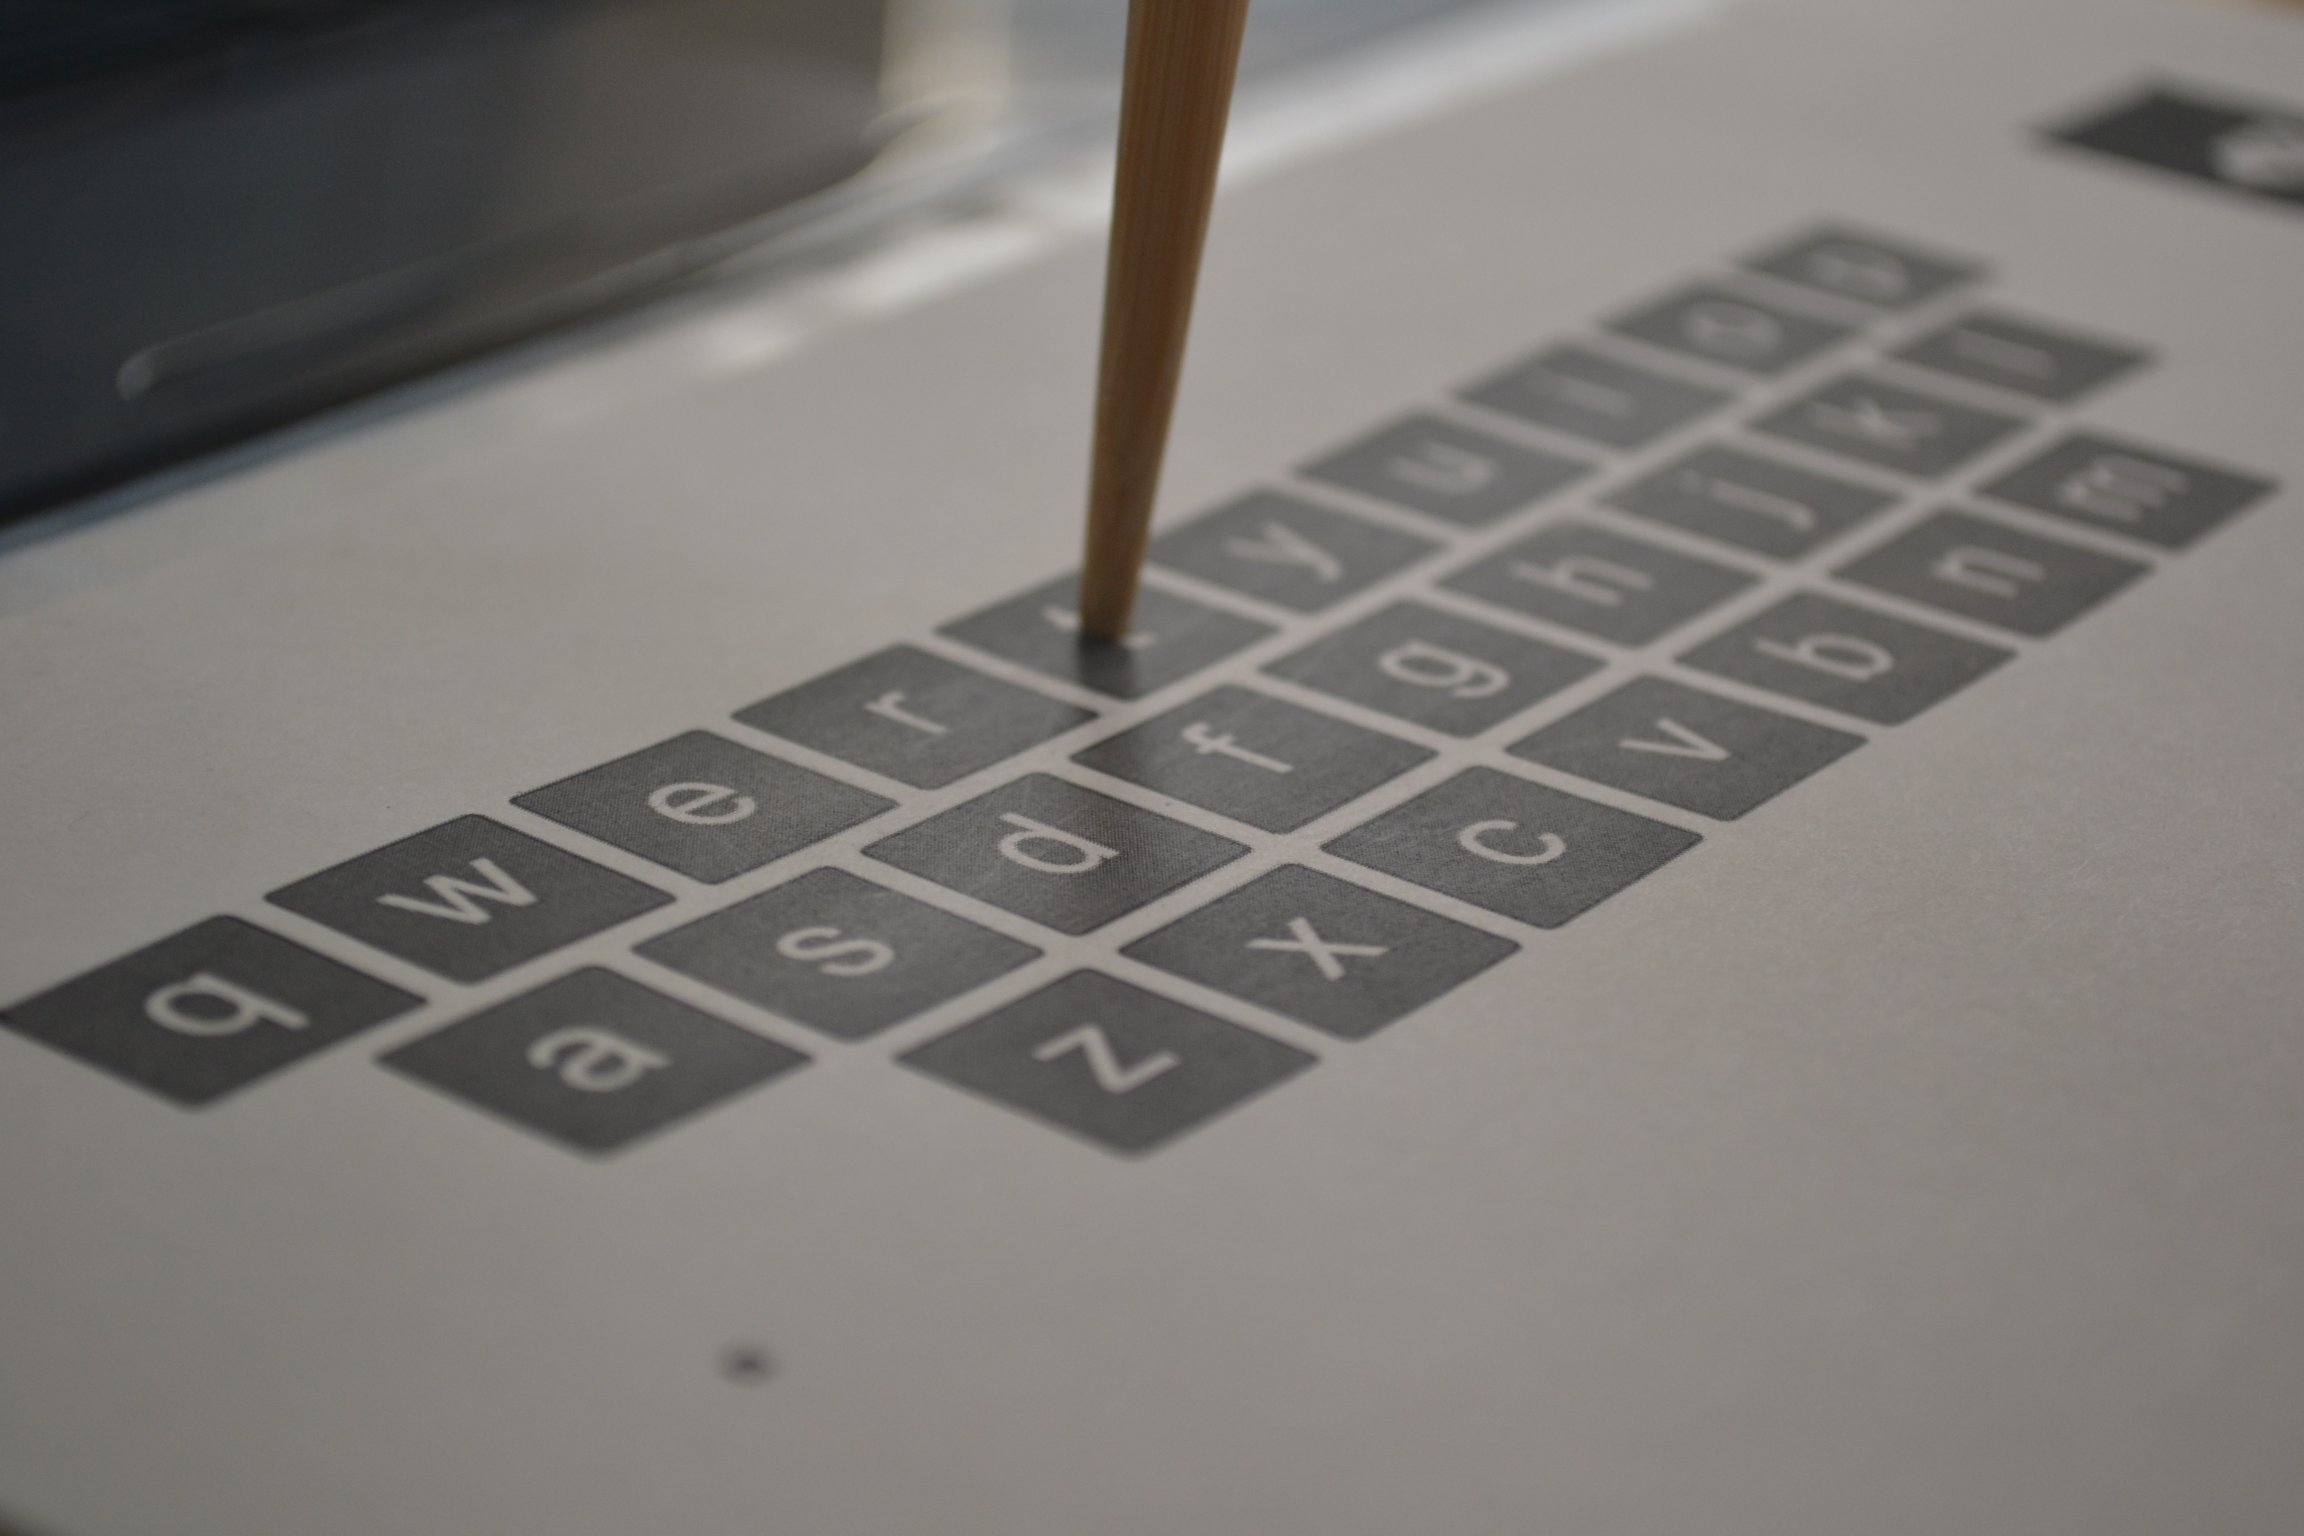
\includegraphics[width=2.9in]{Figures/fig_surface_touch}
		\end{minipage}
	\end{minipage}
	\caption[Leap Surface Word Separation]{A touch was simulated when the stylus hits the paper surface.}
	\label{leap_surface_press_comparison}
\end{figure}

\subsubsection{Size of the motor space}
Figure~\ref{fig_calibration_surface} shows the average calibrated motor space for the Leap Surface Keyboard. The average keyboard was 22.28x5.41 $cm$, with keys that were 1.50x1.50 $cm$ and gaps between keys of 0.23 $cm$.

\subsection{Leap Static-air Keyboard} \label{static_air}
\subsubsection{Interaction method}
The Leap Static-air Keyboard used the Leap Motion controller to track the pointer finger of either hand for interaction. It was designed to simulate a virtual touch screen in mid-air by projecting a quadrilateral plane directly above the interactive surface. The pointer finger would then be used to penetrate the plane to simulate touch.

\subsubsection{Word separation}
Word separation for the Leap Static-air Keyboard worked in a similar way as any ordinary touch-based word-gesture keyboard, However, the simulated touch plane was in mid-air. Touch was simulated by using either pointer finger and penetrating the mid-air interaction plane as seen in Figure~\ref{static_press_comparison}. While maintaining the intersection, the pointer finger was used to draw the word-gesture. By pulling the finger away from the mid-air interaction plane, touch was released.

\begin{figure}[!t]
	\centering
	\begin{minipage}[t]{5.8in}
		\begin{minipage}[t]{2.85in}
			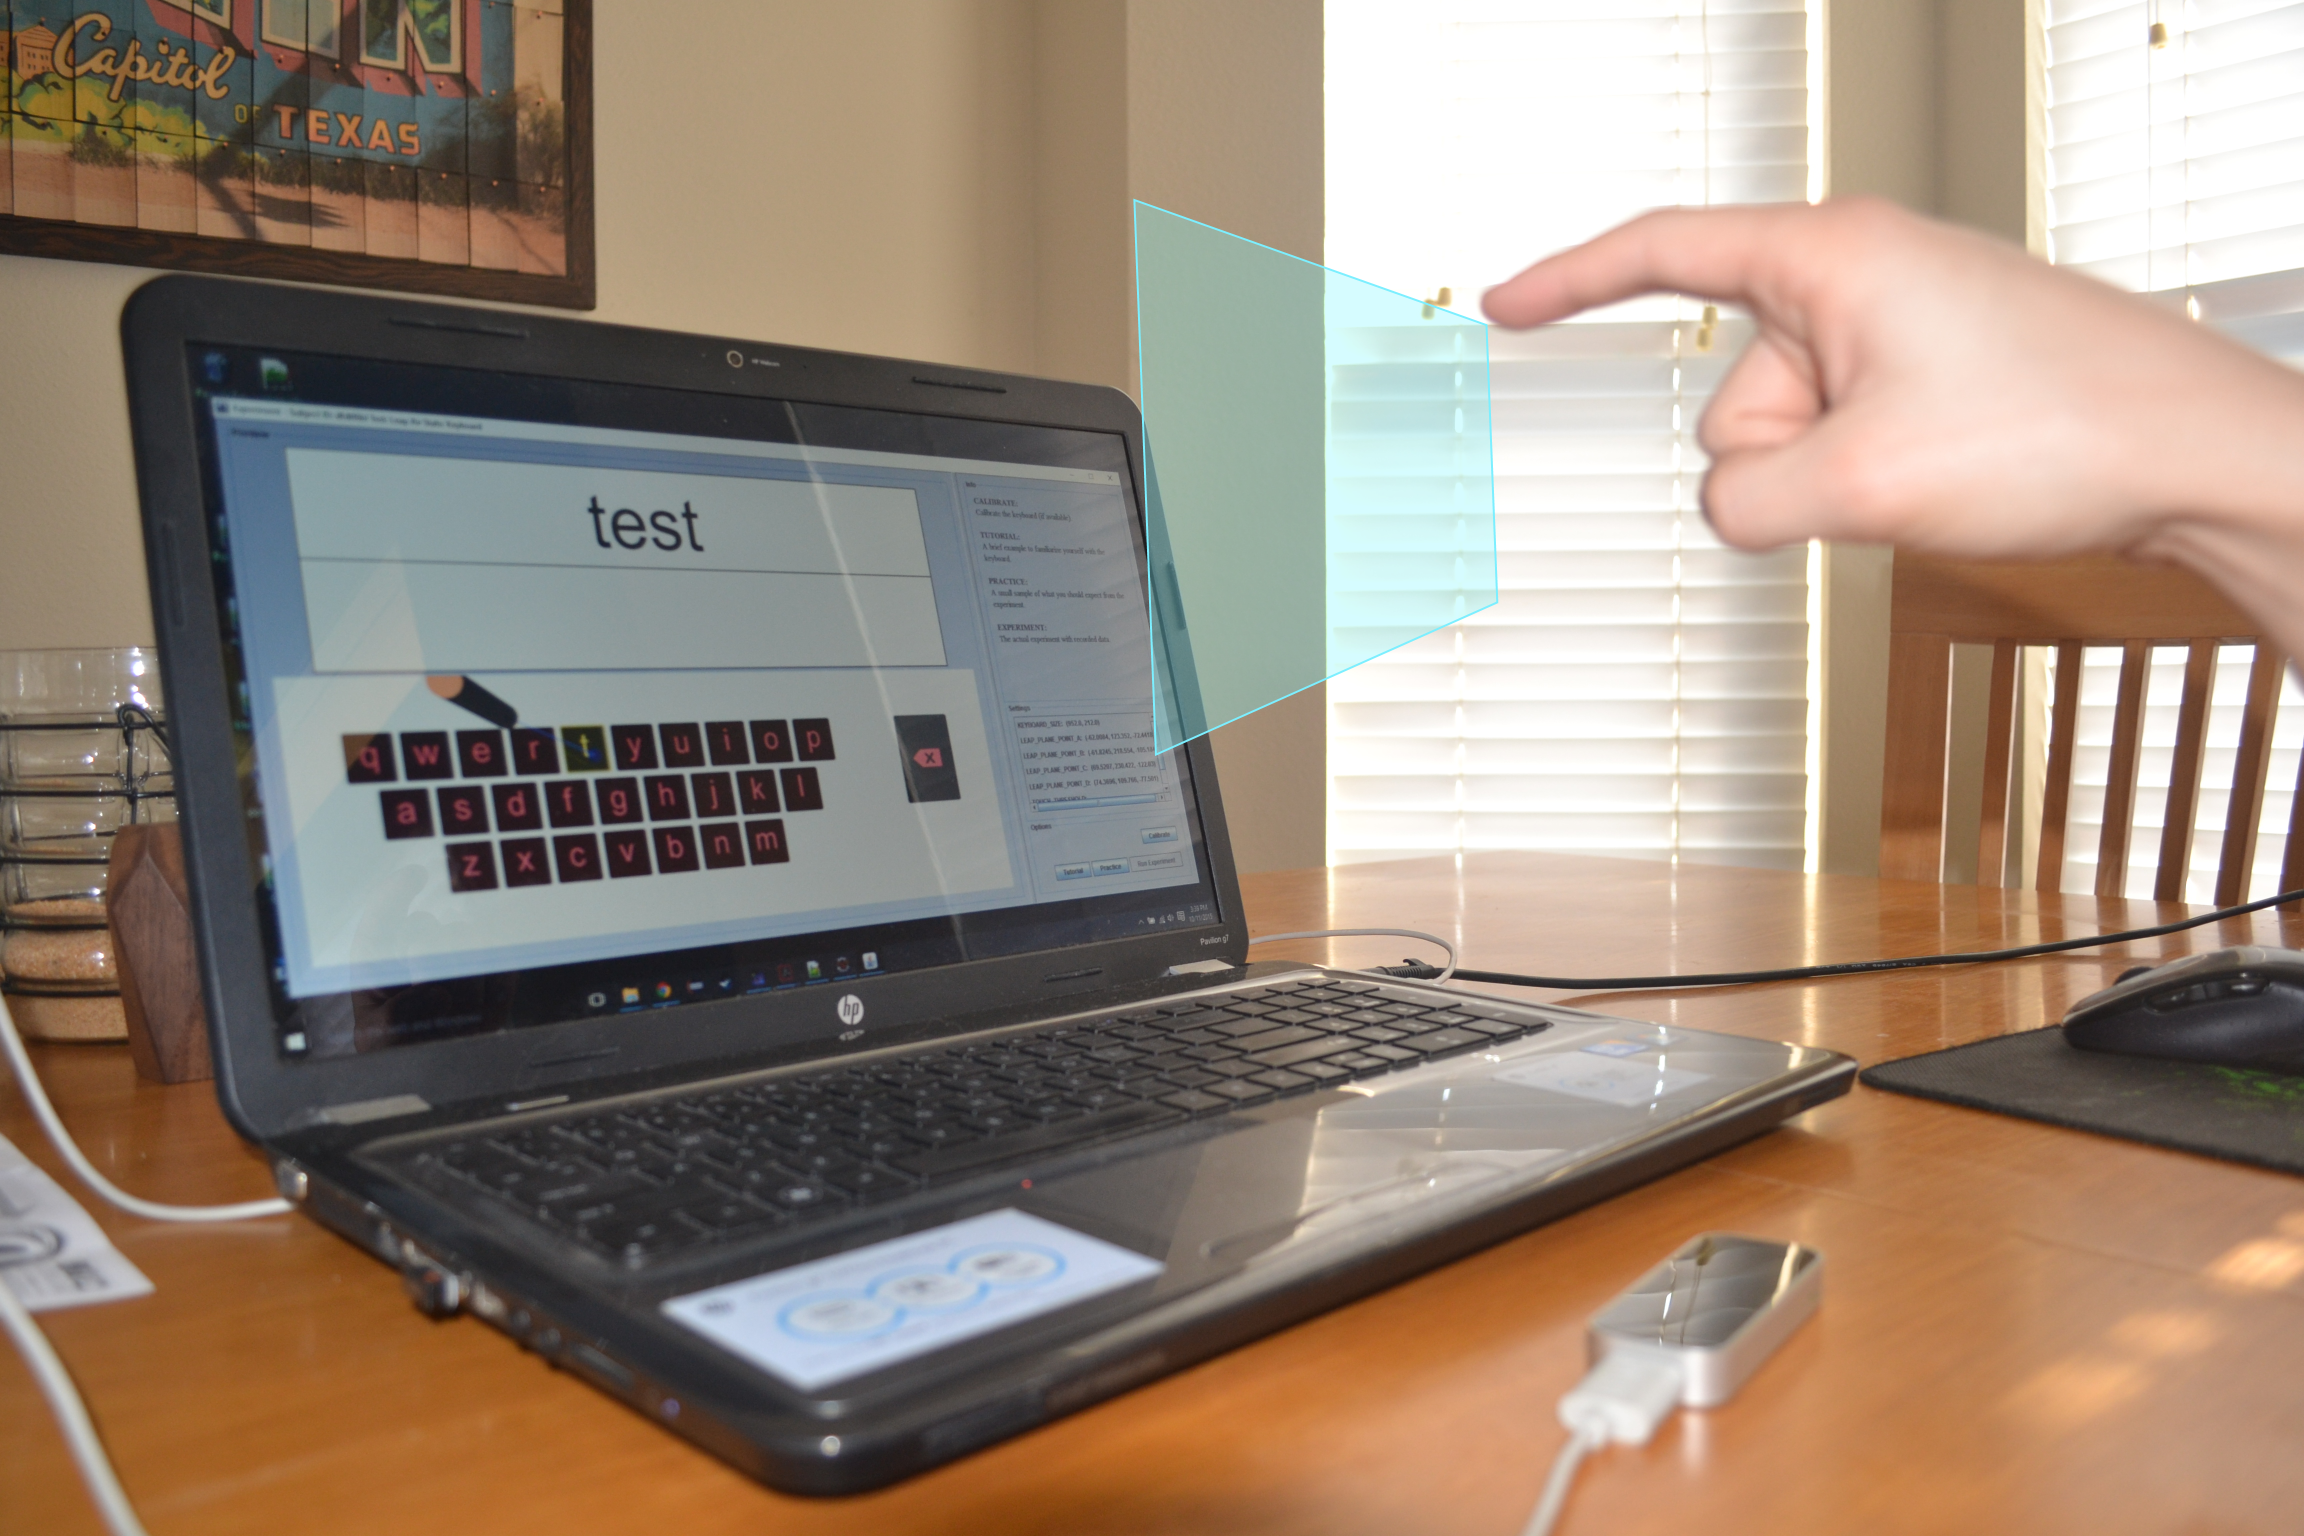
\includegraphics[width=2.9in]{Figures/fig_static_hover}
		\end{minipage}
		\begin{minipage}[t]{2.9in}
			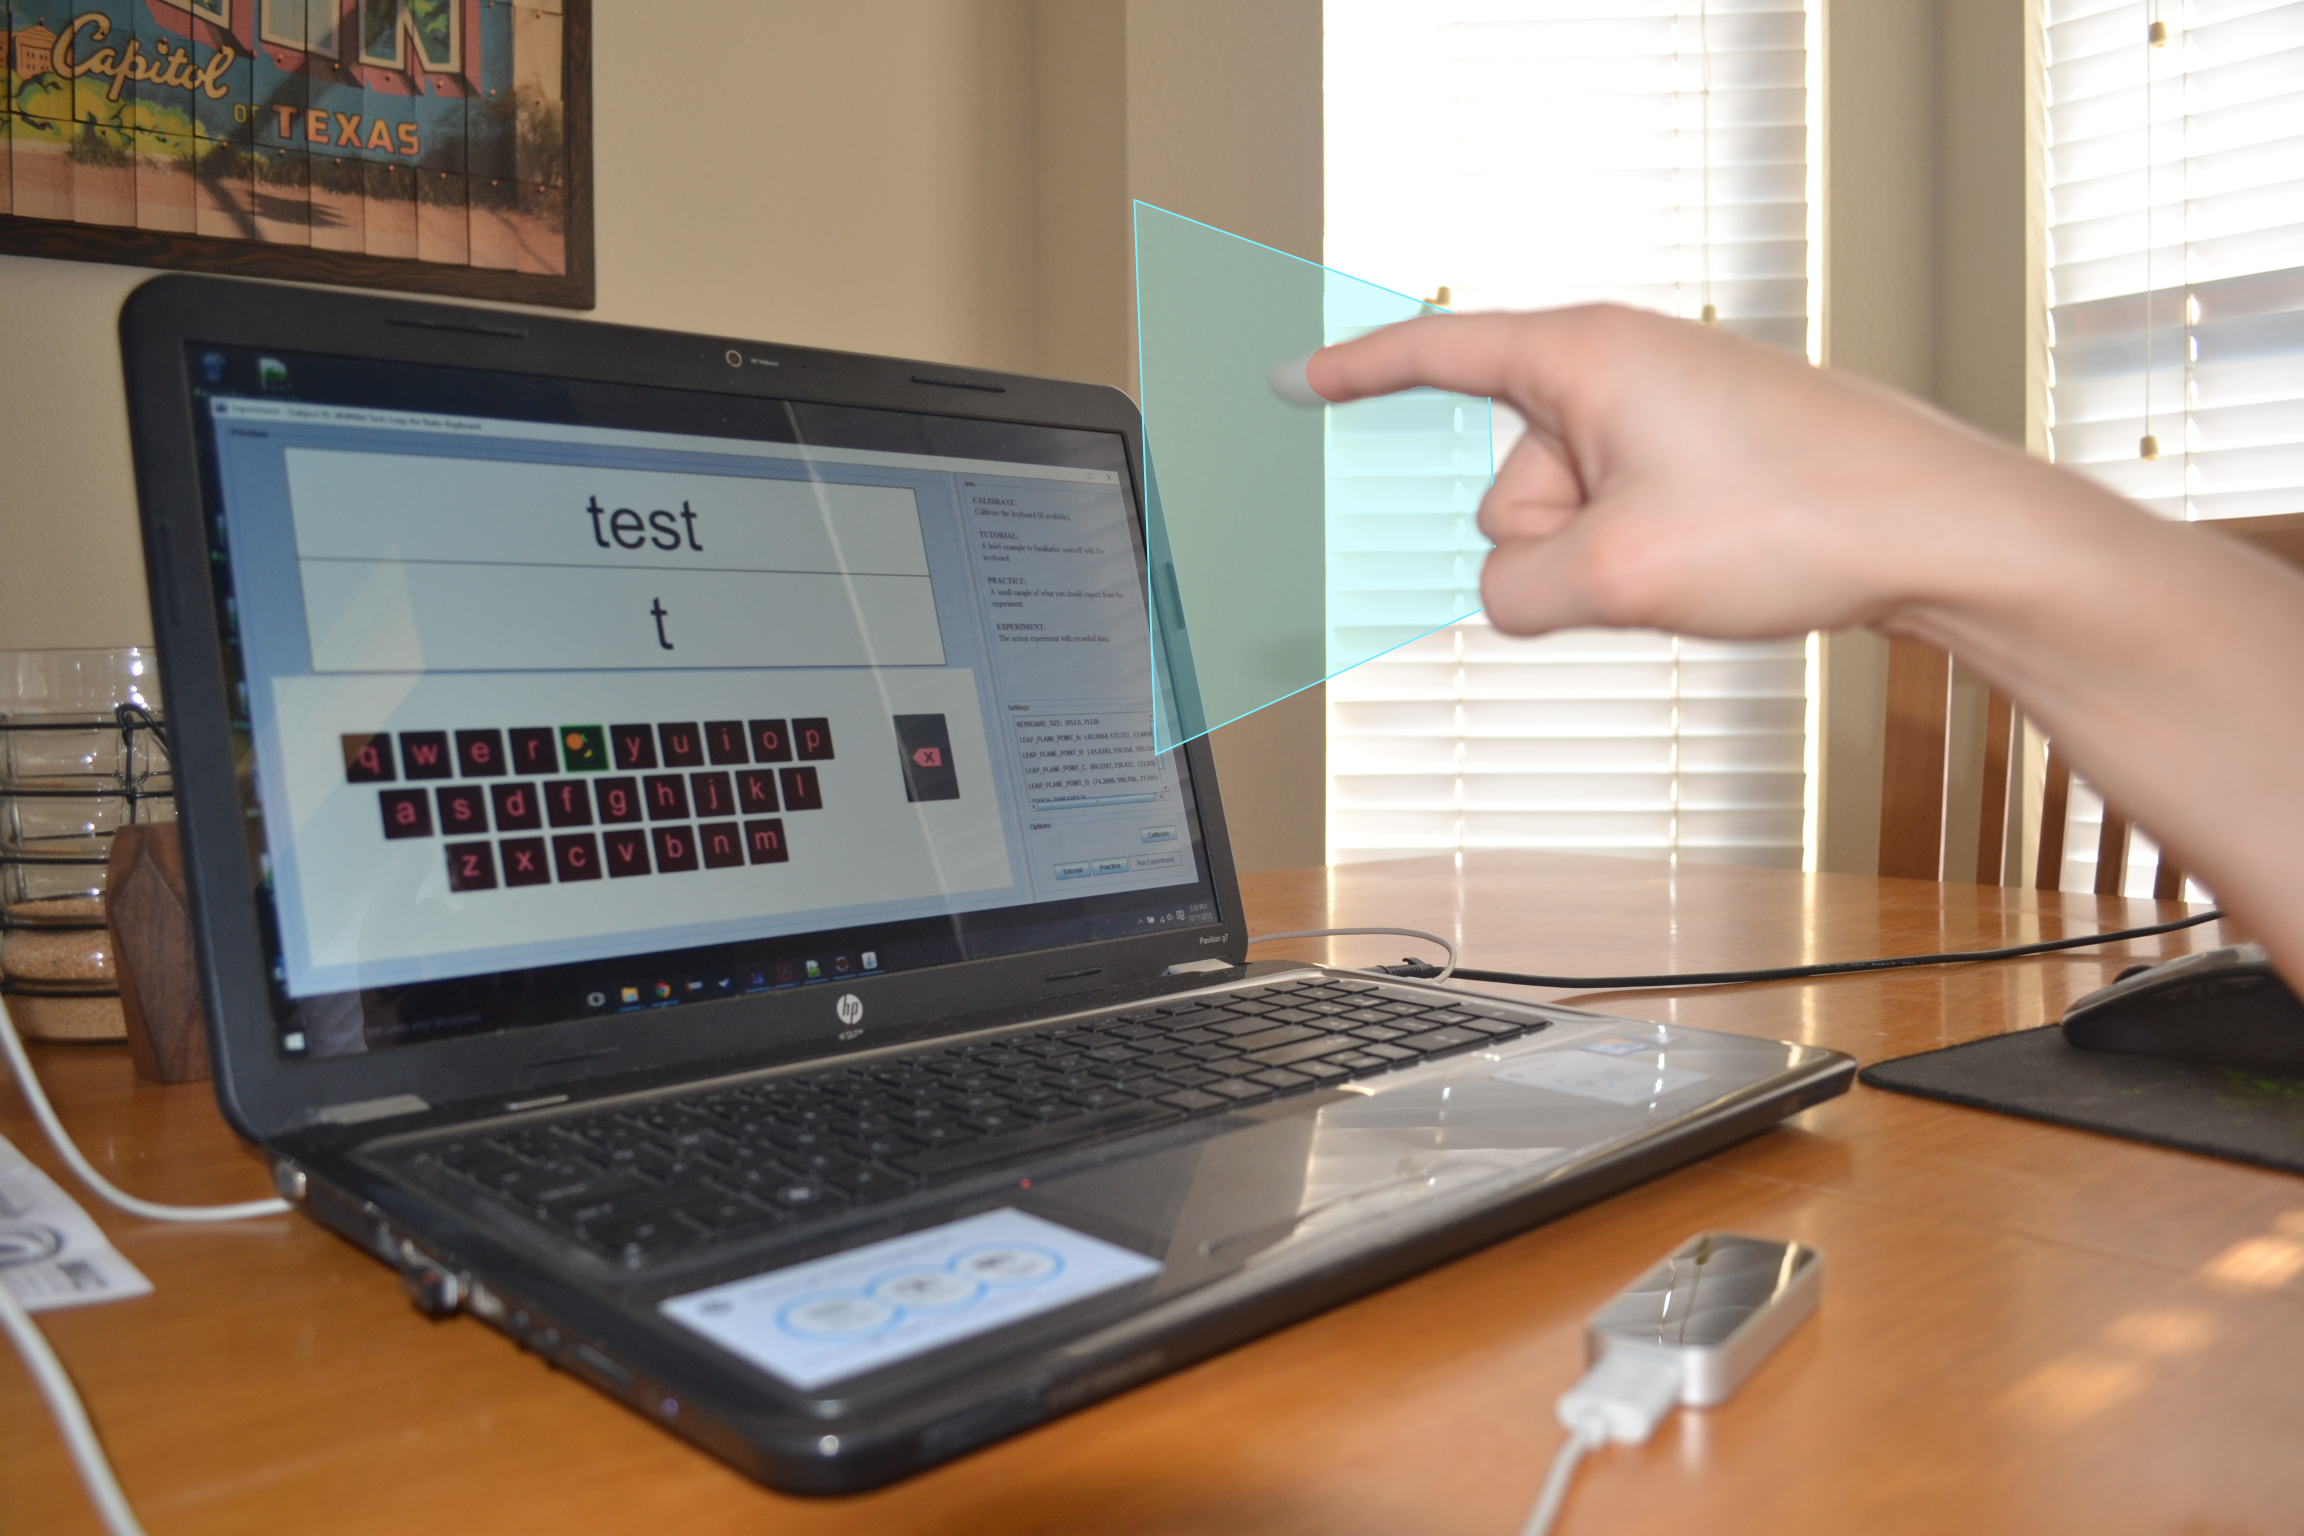
\includegraphics[width=2.9in]{Figures/fig_static_touch}
		\end{minipage}
	\end{minipage}
	\caption[Leap Static-air Word Separation]{A touch was simulated by penetrating the interaction plane.}
	\label{static_press_comparison}
\end{figure}

\subsubsection{Size of the motor space}
Figure~\ref{fig_calibration_static} shows the average calibrated motor space for the Leap Static-air Keyboard. The average keyboard was 13.71x10.07 $cm$, with keys that were 0.92x0.92 $cm$ and gaps between keys of 0.14 $cm$, the same as the Predictive-air and Bimodal-air keyboards.

\subsection{Leap Predictive-air Keyboard} \label{predictive_air_keyboard}
\subsubsection{Interaction method}
The Leap Predictive-air Keyboard used the Leap Motion controller to track the pointer finger of either hand for interaction. It was designed to simulate a virtual touch screen by projecting a quadrilateral plane in the air. However, instead of having to interact with a static, unchanging plane, the Predictive-air Keyboard associates the interaction plane with the participant's pointer finger. As the pointer finger moves forward or backward, the plane follows. By analyzing forward and backward hand gestures in the $z$-direction, the Predictive-air Keyboard tries to move the interaction plane to the pointer finger by predicting when a touch was simulated. Slow gestures serve mostly to move the plane, whereas quick gestures generally snap the plane to the pointer finger. The Leap Motion API provided the predictor values for forward and backward hand gestures.

\subsubsection{Word separation}
Word separation for the Predictive-air Keyboard worked in a similar way as any ordinary touch-based word-gesture keyboard. However, the simulated touch plane was in mid-air. This plane was kept at a consistent distance away from the tracked pointer finger until a forward hand gesture was detected, simulating a touch. The pointer finger could then be used to draw the word-gesture until it was completed. Finally, by making a backward hand gesture away from the interaction plane, the simulated touch was released. The plane interaction was visually similar to Figure~\ref{static_press_comparison}, the Leap Static-air Keyboard interaction.

\subsubsection{Size of the motor space}
Figure~\ref{fig_calibration_static} shows the average calibrated motor space for the Leap Predictive-air Keyboard. The average keyboard was 13.71x10.07 $cm$, with keys that were 0.92x0.92 $cm$ and gaps between keys of 0.14 $cm$, the same as the Static-air and Bimodal-air keyboards.

\subsection{Leap Bimodal-air Keyboard}
\subsubsection{Interaction method}
The Leap Bimodal-air Keyboard was designed to utilize two inputs: the Leap Motion controller and a standard keyboard. The Leap Motion controller tracked the pointer finger of either hand by projecting a quadrilateral plane in the air and snapping the movements of the pointer finger to the plane. A touch was simulated by using the secondary input; in this case, a standard keyboard's space bar.

\subsubsection{Word separation}
In order to move from one word to the next for the Leap Bimodal-air Keyboard, the user activated a secondary input: the standard keyboard's space bar. The interaction plane for simulated touch, as seen in Figure~\ref{bimodal_press}, was still projected in mid-air. Touch was simulated by using either pointer finger to determine the position over the interaction plane in the $x$ and $y$ directions and then by pressing and holding the space bar. While holding down the space bar, the pointer finger was used to draw the word-gesture and finally the space bar was released to end the touch.

\begin{figure}[!t]
	\centering
	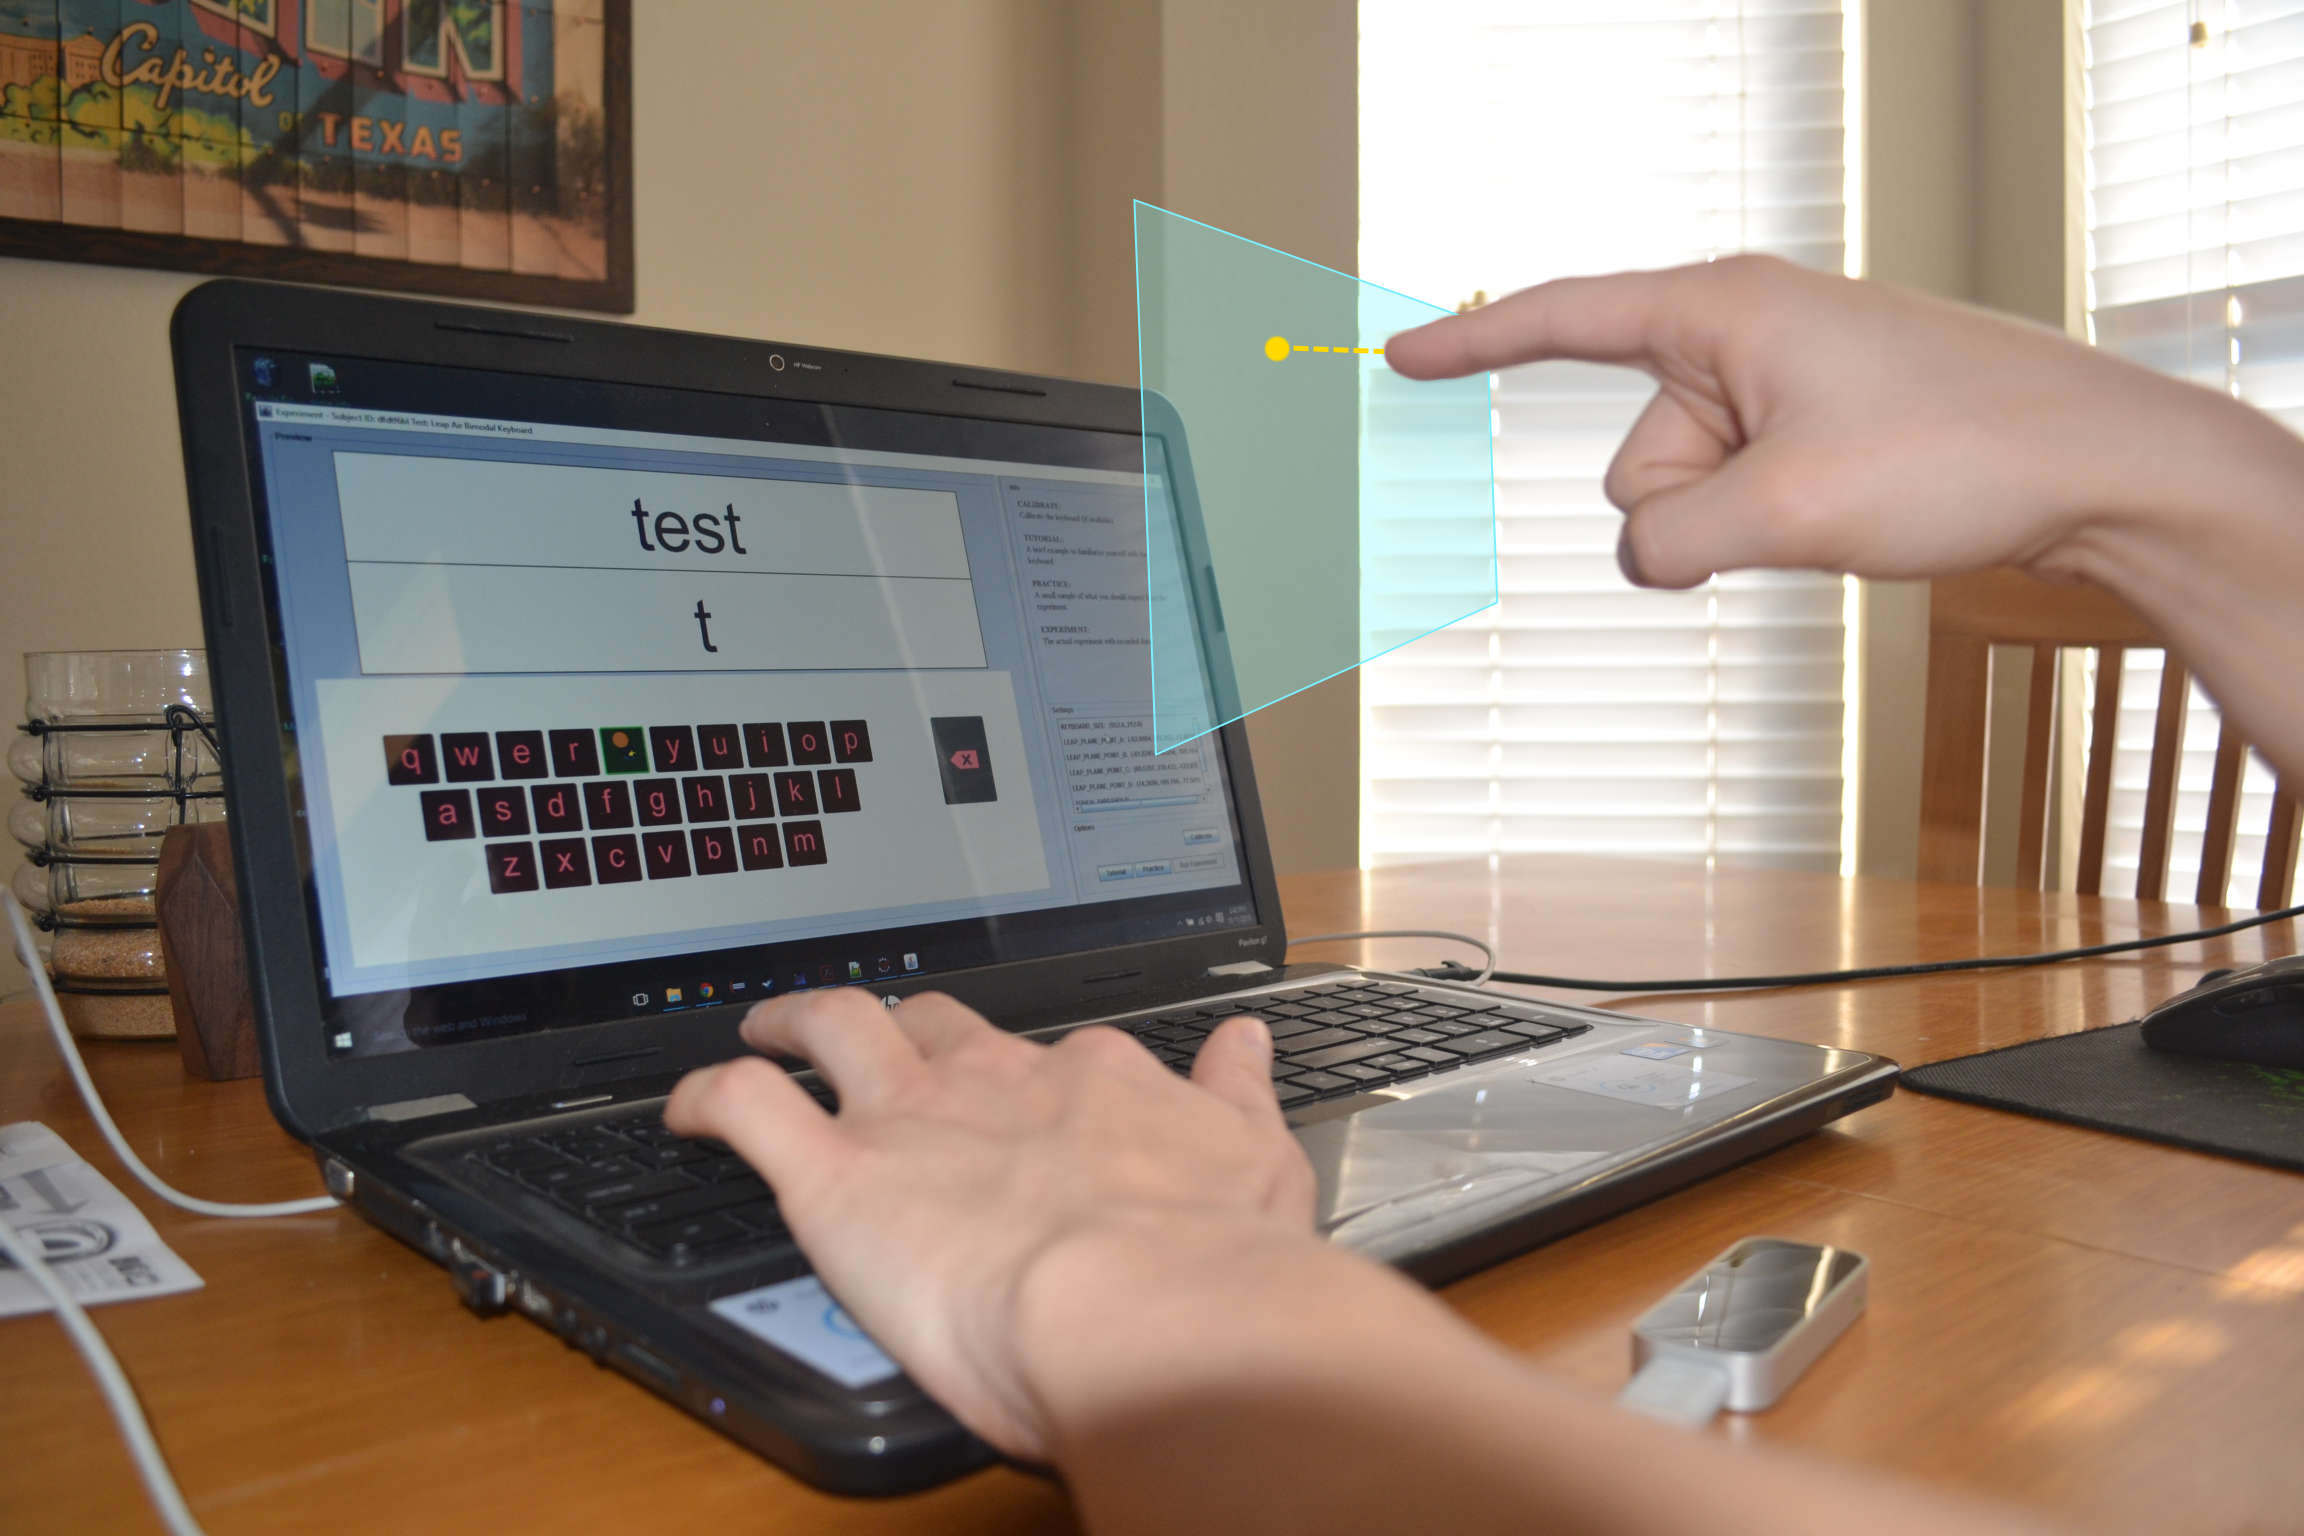
\includegraphics[width=5in]{Figures/fig_leap_bimodal}
	\caption[Leap Bimodal-air Word-separation]{A touch was simulated by pressing the space bar on the keyboard.}
	\label{bimodal_press}
\end{figure}

\subsubsection{Size of the motor space}
Figure~\ref{fig_calibration_static} shows the average calibrated motor space for the Leap Bimodal-air Keyboard. The average keyboard was 13.71x10.07 $cm$, with keys that were 0.92x0.92 $cm$ and gaps between keys of 0.14 $cm$, the same as the Static-air and Predictive-air keyboards.

\subsection{Leap Pinch-air Keyboard}
\subsubsection{Interaction method}
The Leap Pinch-air Keyboard used the Leap Motion controller to track the palm of either hand for interaction. It was designed to project a quadrilateral plane in mid-air and snapped the palm position to the plane in the $z$-direction. The hand could then be used to form a pinch-gesture to simulate touch. The Leap Motion API provided the predictor values for recognizing pinching-gestures. It is important to note that unlike in Vulture \cite{ref_vulture}, no glove was required and many different pinch-gestures were recognized.

\subsubsection{Word separation}
A pinching-gesture was used to move to the next word in the sequence for the Leap Pinch-air Keyboard. However, the interaction plane was still projected in mid-air. Touch was simulated by using either hand and then forming and holding a pinching-gesture, as shown in Figure~\ref{pinch_press_comparison}. While pinching, the word-gesture was drawn and then released to end the ``touch.''

\subsubsection{Size of the motor space}
Figure~\ref{fig_calibration_pinch} shows the average calibrated motor space for the Leap Pinch-air Keyboard. The average keyboard was 16.86x9.04 $cm$, with keys that were 1.13x1.13 $cm$ and gaps between keys of 0.18 $cm$.

\begin{figure}[h]
	\centering
	\begin{minipage}[t]{5.8in}
		\begin{minipage}[t]{2.85in}
			\includegraphics[width=2.9in]{Figures/fig_pinch_hover}
		\end{minipage}
		\begin{minipage}[t]{2.9in}
			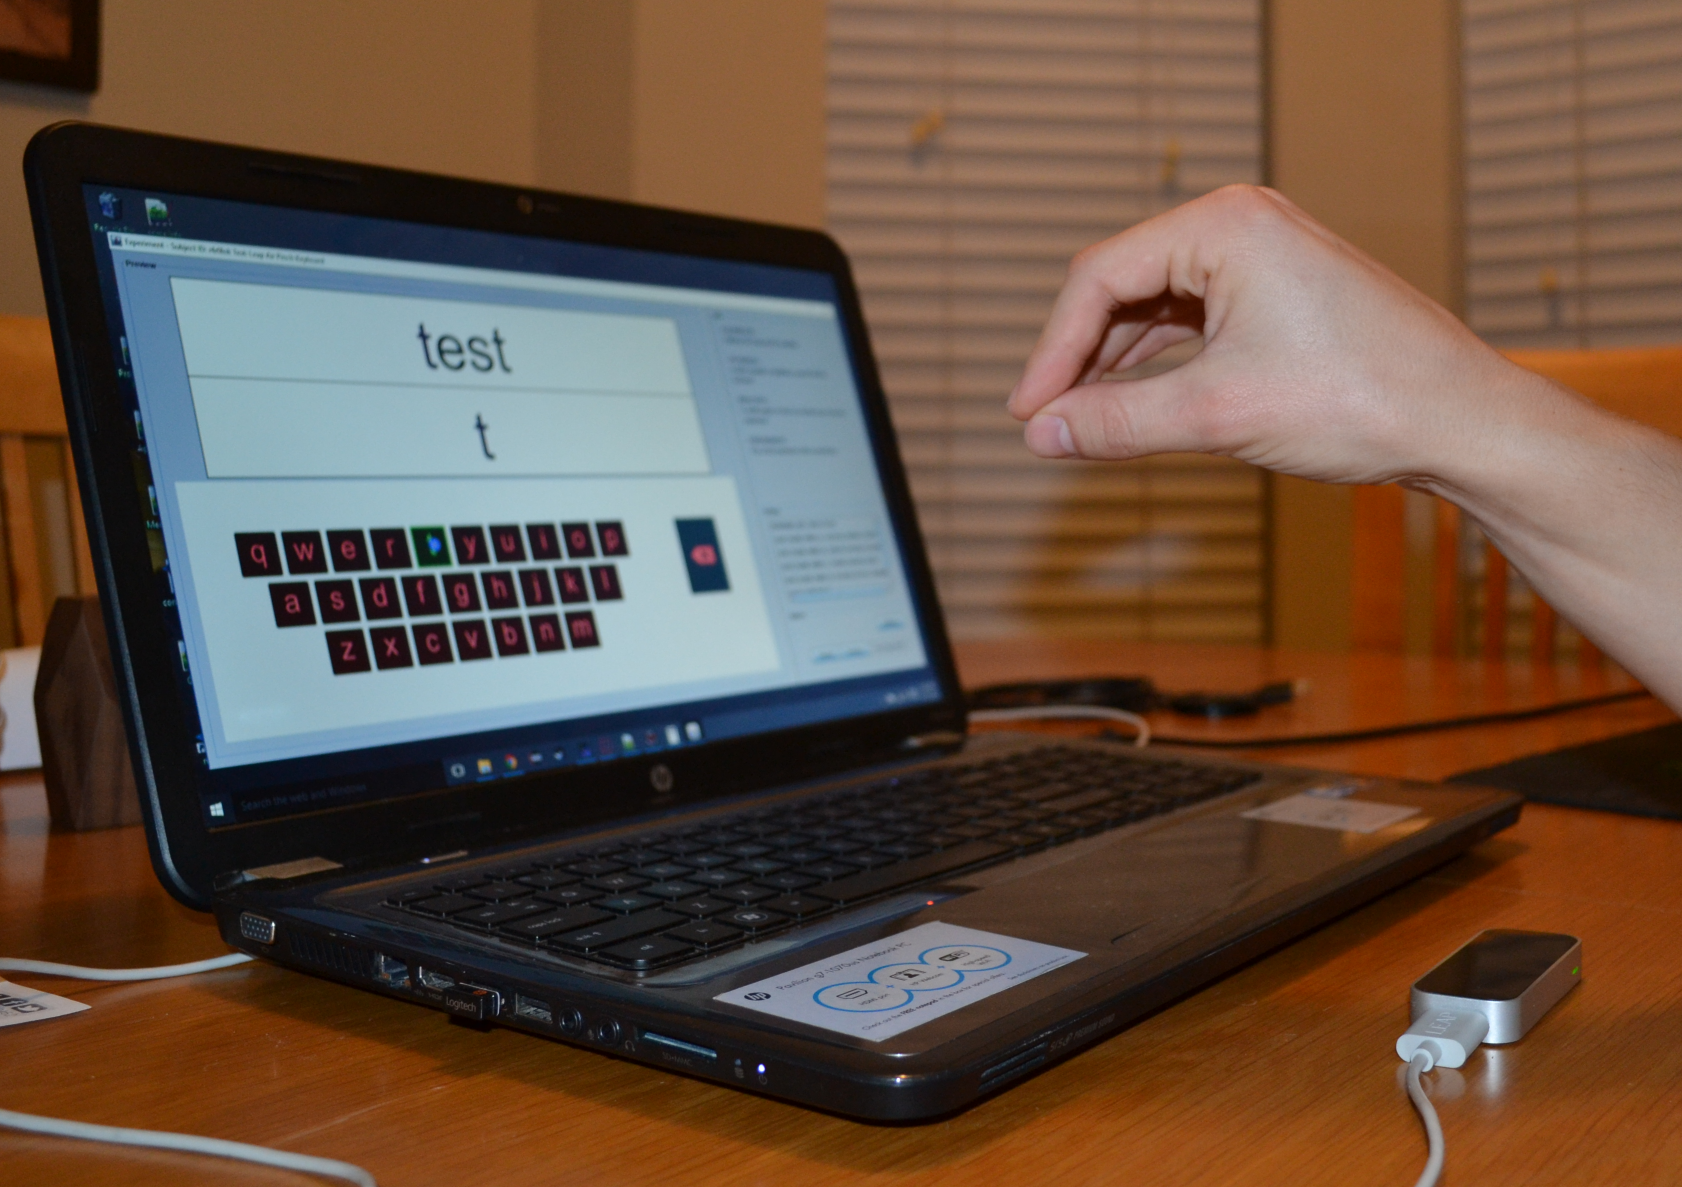
\includegraphics[width=2.9in]{Figures/fig_pinch_touch}
		\end{minipage}
	\end{minipage}
	\caption[Leap Pinch-air Word Separation]{A touch was simulated by making a pinching gesture.}
	\label{pinch_press_comparison}
\end{figure}